%-----------------------------------------------------------------------------------------------------
\chapter{Materials and Methods}
\label{chap:materials_methods}
%-----------------------------------------------------------------------------------------------------


Following the review of commercial systems and research initiatives discussed previously, this chapter presents the practical implementation of a low-cost antenna radiation pattern measurement system. Designed to meet educational and experimental needs around the 868 MHz ISM band, the proposed setup combines mechanical design, custom electronics, and software integration. This chapter describes the materials used, the configuration of each subsystem, and the validation methodology. Additionally, it highlights RF-related improvements, including a custom-designed air-core choke balun and an impedance matching network.
\vspace{0.1em}

%-----------------------------------------------------------------------------------------------------
\section{Proposed System Description}
\label{sec:system_description}
%-----------------------------------------------------------------------------------------------------

The antenna radiation pattern measurement system was developed with an emphasis on low cost, modularity, and suitability for educational and experimental applications. Built using commercially available components and custom-fabricated parts, the system allows for easy replication and future enhancements. It is composed of the following main subsystems:

\begin{itemize}
    \item \textbf{Mechanical substructure} with two independent rotational axes (azimuth and perpendicular) for the receiving antenna.
    \item \textbf{Electronic control system} based on the ATmega328P microcontroller (Arduino Uno).
    \item \textbf{RF power measurement circuit} using the AD8313 logarithmic detector.
    \item \textbf{MATLAB software suite} for motor control, data acquisition, and real-time visualization.
\end{itemize}

\subsection{System Architecture}
\label{subsec:system_architecture}

The system includes two rotational axes: the azimuth axis, located at the base, and a perpendicular axis at the top, which enables angular scanning in an orthogonal plane. Depending on the antenna mounting orientation, this perpendicular axis can be adapted to perform elevation, as shown in Figure \ref{cap3:sec1:fig1}. Both axes are actuated by NEMA 17 stepper motors with $1.8^\circ$ step angle, driving belt-and-pulley mechanisms. To prevent twisting of the coaxial cable and transmission wires, the motor moves up to $180^\circ$ in one direction, returns to the home position, and then moves up to $180^\circ$ in the opposite direction.

\begin{figure}[H]
    \centering
    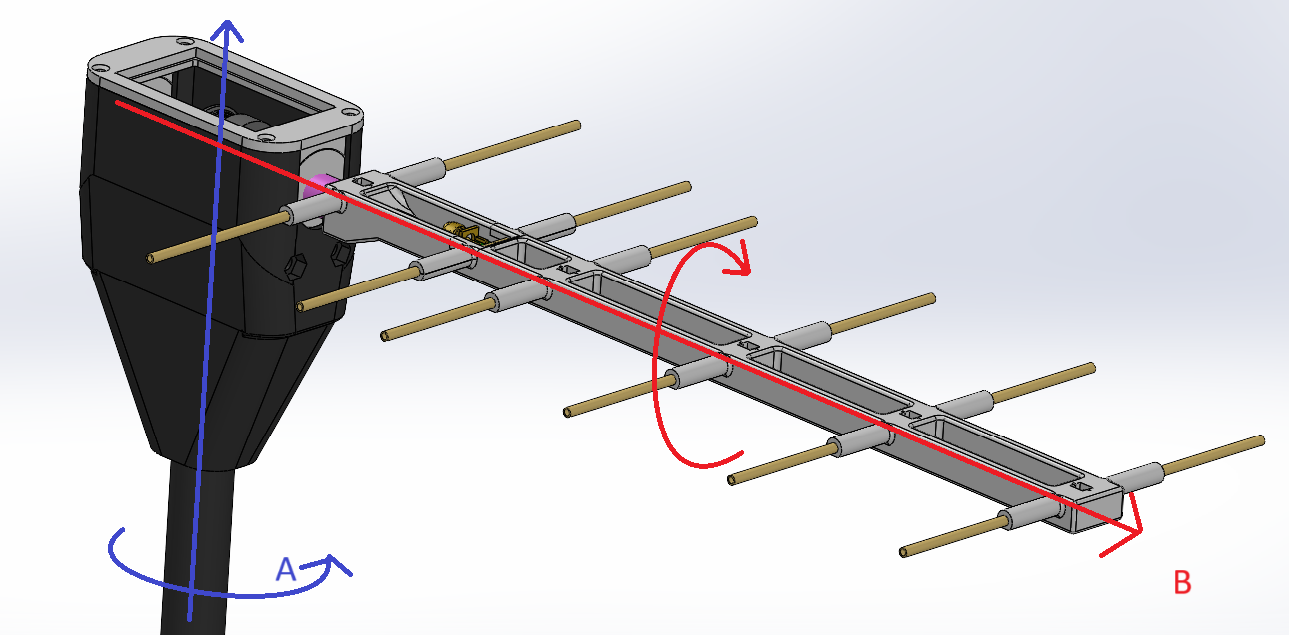
\includegraphics[width=0.85\textwidth]{Imagens/antenna_rotation.png}
    \caption{CAD model of the rotating platform with two degrees of freedom. Axis ``A'' corresponds to the azimuth rotation and axis ``B'' to the perpendicular rotation, which can be configured as the elevation axis.}
    \label{cap3:sec1:fig1}
\end{figure}

The mechanical transmission system, based on belts and polies, was specifically designed to achieve a resolution of approximately $1 ^ \circ$ of revolution per motor step. This was achieved by using custom-designed gears with a 1.8:1 ratio. The rotating assembly is supported by low-friction components to ensure smooth motion and reproducibility of measurements.

It is worth noting that despite the mobile platform responsible for rotating the antenna under test, the complete system also includes a fixed structure that acts as a transmitting station. This fixed base has dimensions and construction characteristics similar to the rotational platform, such as mounting height and accommodation of the transmitting antenna. Even without motorised degrees of freedom, the antenna installed on this base can be manually oriented on different axes, allowing for various configurations, such as azimuth or orthogonal alignment, according to the desired experiment. Thus, the assembly consists of two complementary mechanisms, assisting in the measurement of radiation patterns in different scenarios.


\subsection{Components Used}
\label{subsec:components_used}

The main components used in the construction of the system are:

\begin{itemize}
 \item \textbf{Stepper Motors}: NEMA 17 bipolar stepper motors with $1.8 ^ \circ$ per step, configured for 1/16 microstepping using DRV8825 drivers. These motors were selected over commun low-cost servo motors due to their superior precision and high torque, which are crucial for achieving accurate angular positioning required for antenna pattern measurements. 
\item \textbf{Microcontroller}: Arduino Uno board, based on the ATmega328P, is responsible for coordinating motor motion, executing homing routines, and reading sensor data. The Arduino Uno was chosen for its ease of programming, widespread community support, and cost-effectiveness, making it an ideal platform for an educational and experimental system.
 \item \textbf{RF Power Sensor}: Analog Devices AD8313 module, operating from 100~MHz to 2.5~GHz range, with a dynamic range of up to 70~dB. This sensor was selected because it can be supplied inexpensively from the Asian market. %due to its wide operating frequency range and high dynamic range, which are essential for accurately measuring varying RF power levels across the target ISM band of 868 MHz.
\item \textbf{Magnetic Position Sensors}: Hall-effect magnetic sensors (KY-035 49E), used for homing reference detection on each rotational axis. These sensors provide a reliable and low-cost solution for precise homing, ensuring consistent starting positions.
\item \textbf{Power Supply}: Industrial 12~V DC, 2~A power supply (Orno OR-ZL-1631), rated at 24~W with IP20 protection and 230~V Alternating Current (AC) input, providing regulated voltage to all system components. A standard power supply was chosen for its reliability and capability to provide stable and sufficient power to all active components of the system.
\item \textbf{Mechanical Structure}: The platform consists of a one-meter fibreglass tube (non-conductive and lightweight), 3D-printed pulleys and brackets, and a wooden base in circular shape. Non-metallic materials were deliberately selected near the antenna to avoid reflections or distortions by the radiation pattern. Even the internal bearings are from nylon materials. Some components of the mechanical structure, such as the wooden base, were sourced in a manner that did not significantly impact the final cost of the project, further aligning with the low-cost objective. Fibreglass and Polylactic Acid (PLA) were chosen for their non-conductive, lightweight properties, minimizing interference and ensuring the structural integrity of the rotating assembly without affecting RF measurements.
\item \textbf{RF Generator}: It is a handheld RF signal generator which is used as a signal source. It operates in a frequency range from 100 kHz up to 6 GHz, offering both CW (Continuous Wave) and sweep modes, with output power from approximately –60 dBm to +15 dBm. Detailed characterisation of both the signal generator and the antenna systems in transmitter and receiver configurations will be present later.

\end{itemize}

% \subsection{Transmitter}

% It is important to mention that, although a commercial RF source was employed, the transmitting antenna and its support structure are functionally identical to the receiving system. The transmitter is a fixed installation, and has the same non-conductive fibreglass tube support, PLA antenna mount, and wooden base as the receiver.

% A handheld RF Explorer Signal Generator was used as the signal source. The device operates in a frequency range from 100 kHz up to 6 GHz, offering both CW and sweep modes, with output power from approximately –40 dBm to +10 dBm. Detailed characterisation of both the signal generator and the antenna systems in transmitter and receiver configurations will be present later.

%-----------------------------------------------------------------------------------------------------
\section{Electrical Subsystem}
\label{subsec:electrical_subsystem}
%-----------------------------------------------------------------------------------------------------



As illustrated in the block diagram in Figure~\ref{cap3:sec2:fig1:a}, the electrical control system is based on an Arduino Uno board (ATmega328P), combined with a dual stepper motor driver shield. This shield integrates two DRV8825 drivers, each configured for 1/16 microstepping via onboard Dual In-line Package (DIP) switches. It simplifies the electrical connections and consolidates the power and control interfaces for the stepper motors.
\begingroup
\setlength{\textfloatsep}{2pt}
\setlength{\intextsep}{2pt}
\begin{figure}[H]
    \captionsetup{aboveskip=1pt,belowskip=1pt}
     \centering
     \begin{subfigure}{0.48\textwidth}
         \centering
         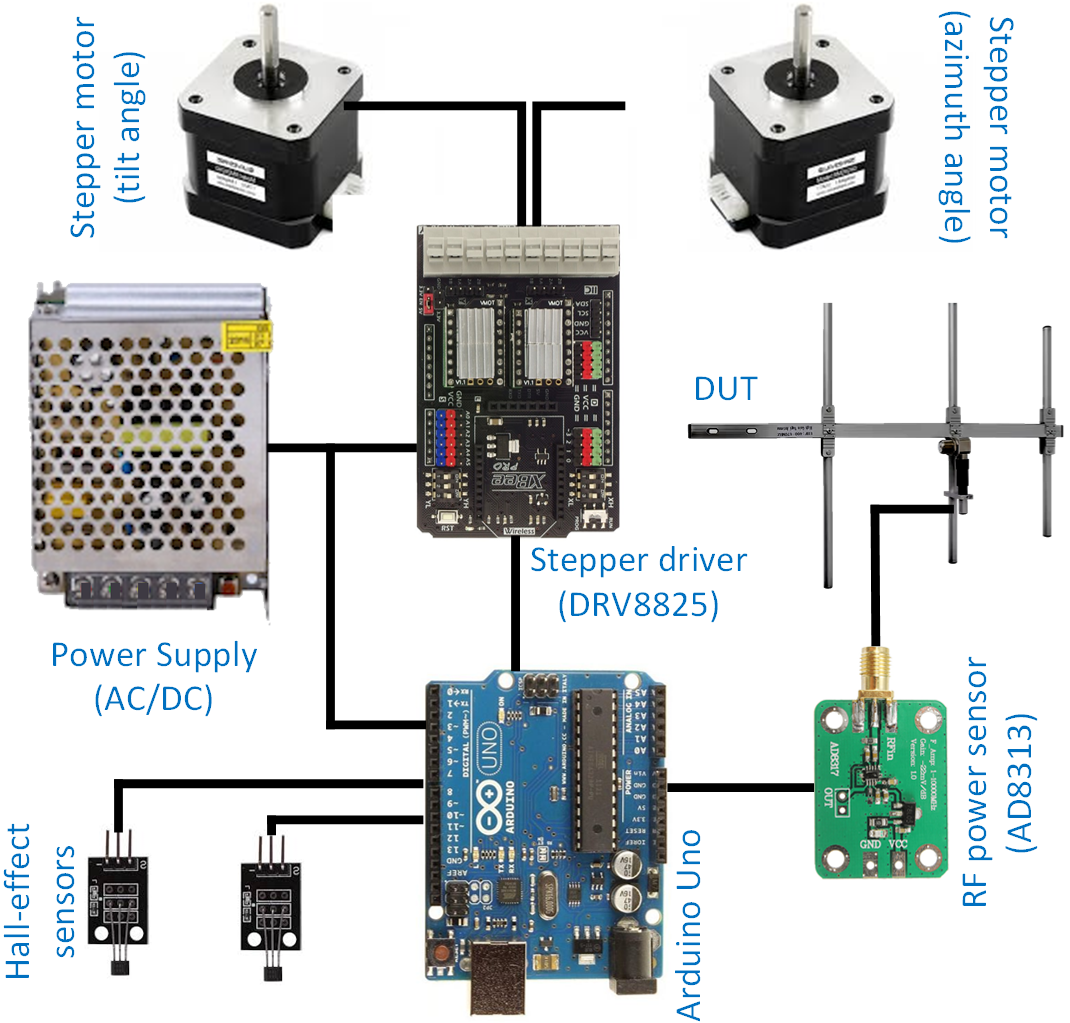
\includegraphics[width=\textwidth]{Imagens/hardware_block_diagram_v2.png}
         \caption{Block diagram of the electrical system}
         \label{cap3:sec2:fig1:a}
     \end{subfigure}
     \hspace{1mm}
     \begin{subfigure}{0.48\textwidth}
         \centering
         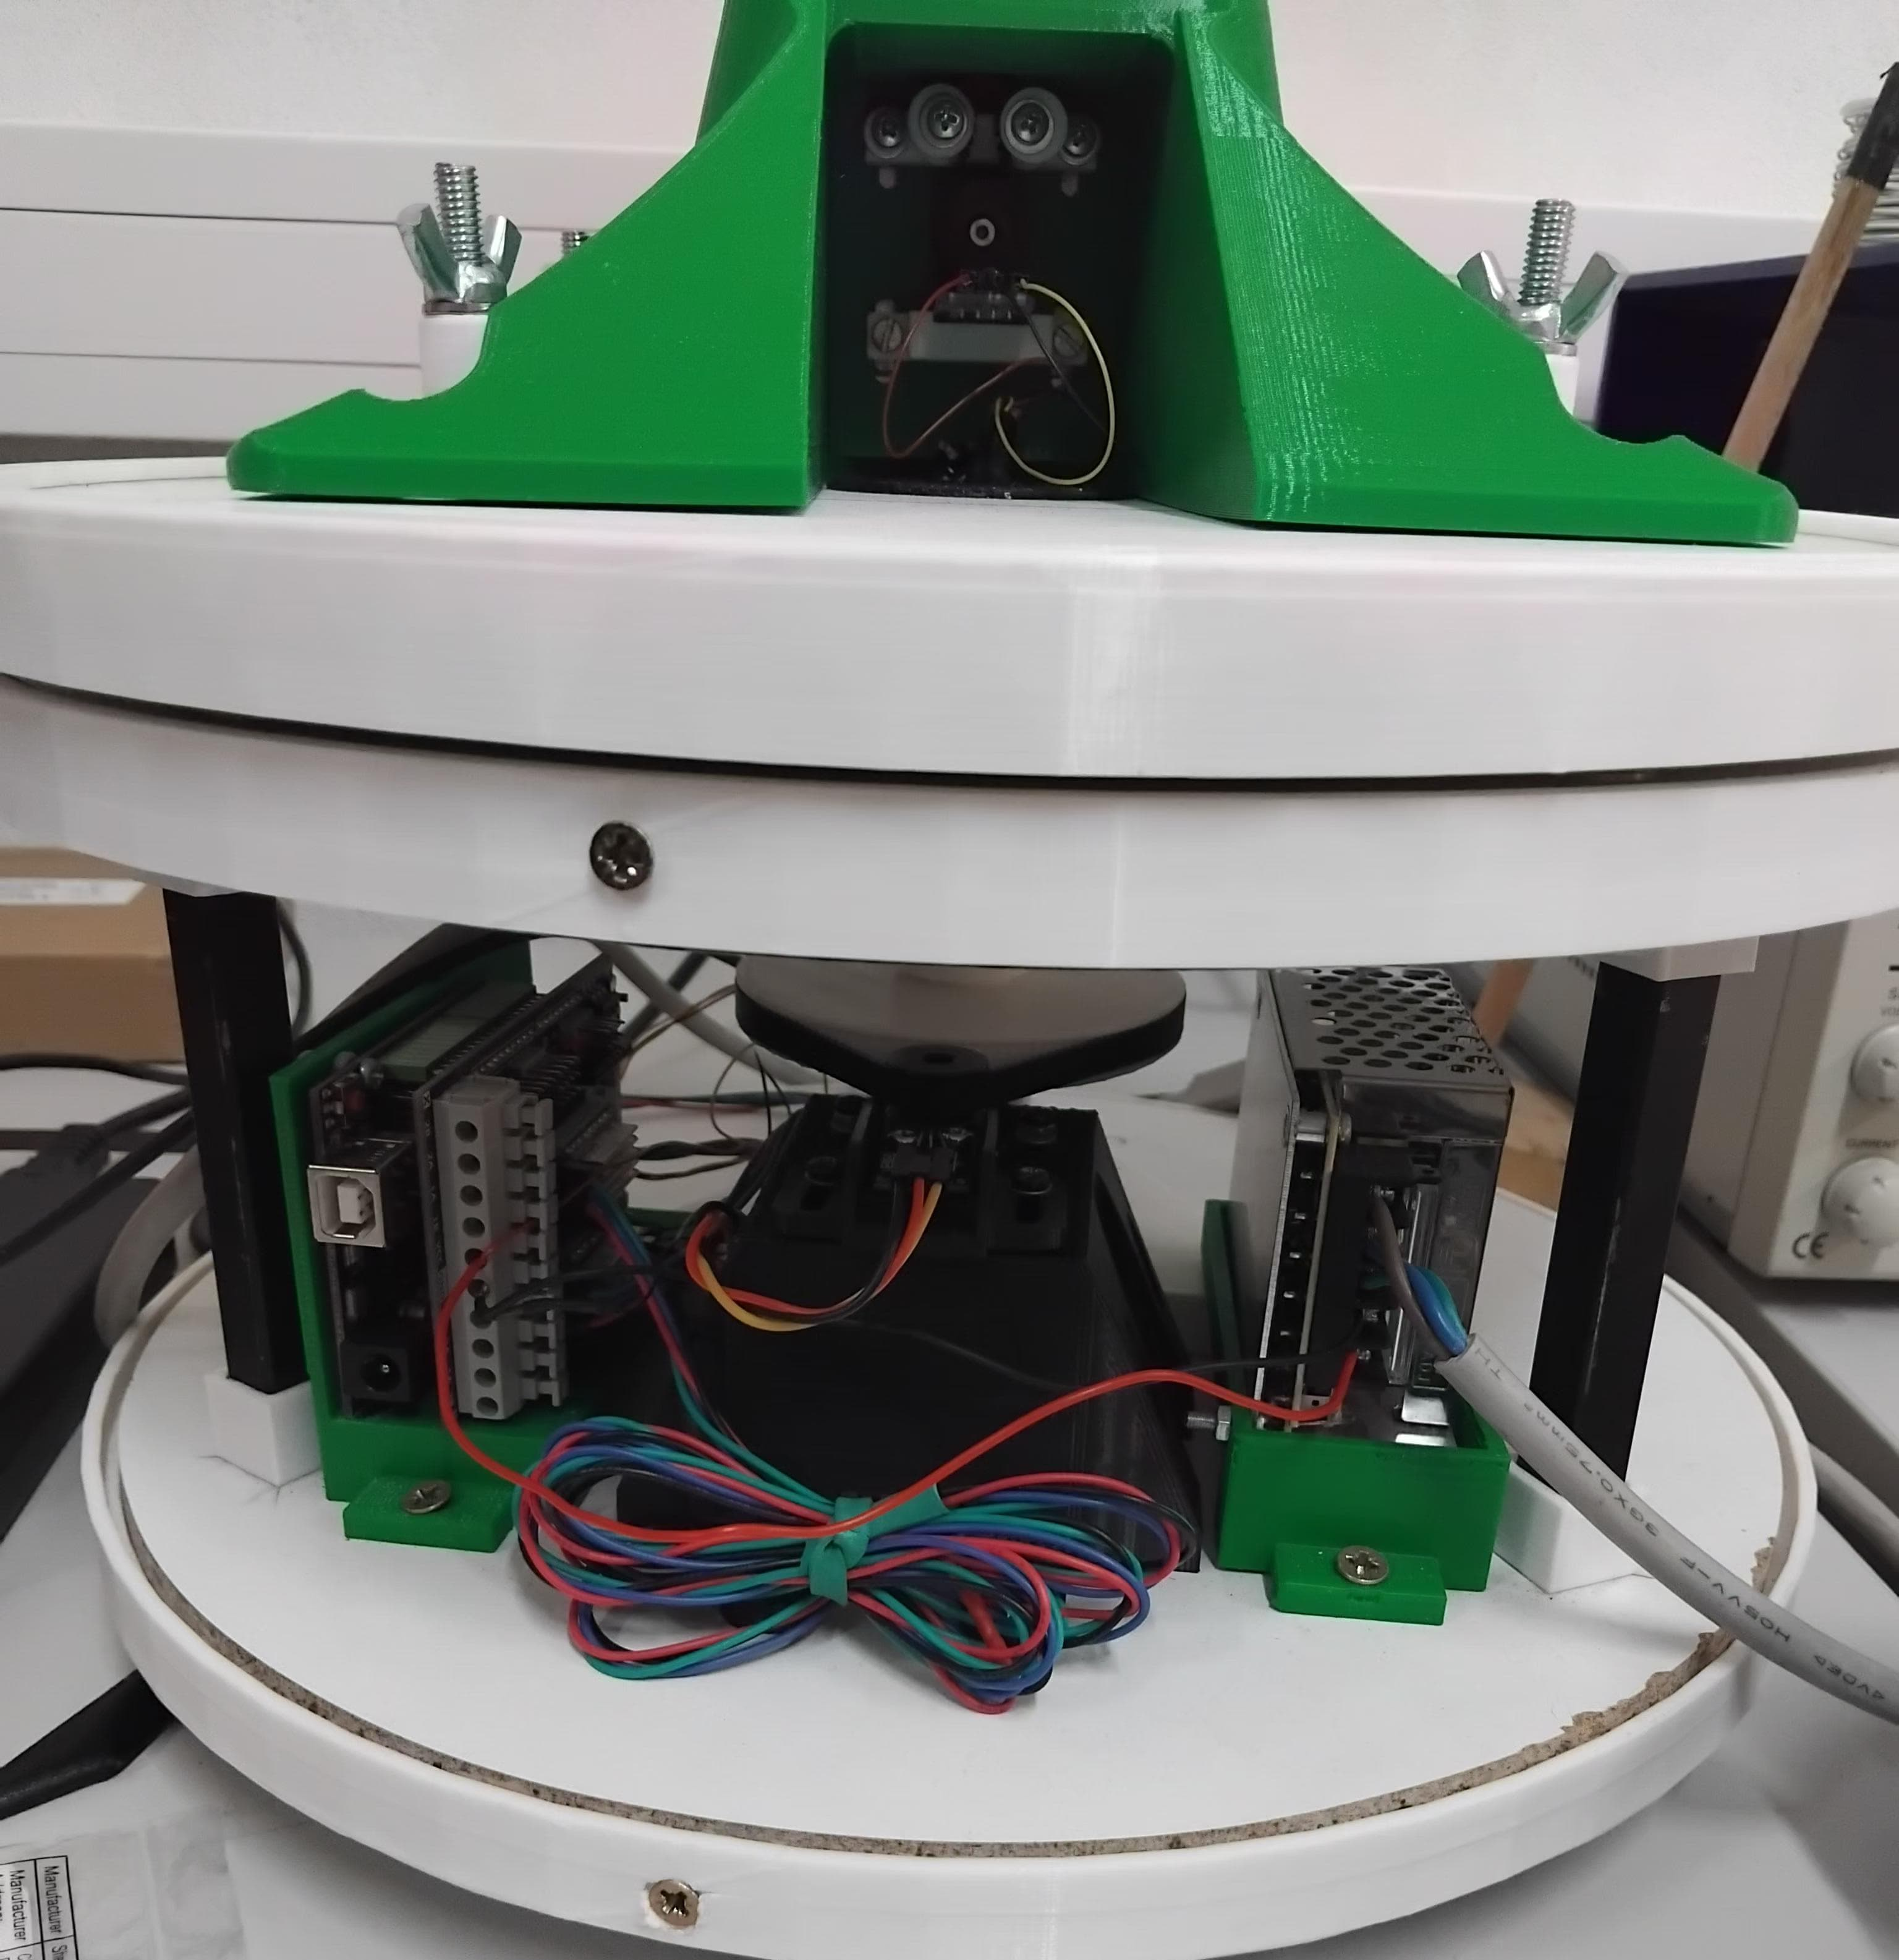
\includegraphics[width=\textwidth]{Imagens/system_real_photo.jpg}
         \caption{Assembled base of the measurement system}
         \label{cap3:sec2:fig1:b}
     \end{subfigure}
        \caption{Block diagram and photo of the electrical system, including key components like the Arduino Uno, DRV8825 driver shield, power supply, sensors, RF detector (AD8313), Device Under Test (DUT), stepper motors, and internal wiring.}
        \label{cap3:sec2:fig1}
\end{figure}
\endgroup
\vspace{-0.1em}

The H-bridge shield receives 12~V from the external power supply, which is then distributes power to the stepper motors and Arduino board. It also powers auxiliary components, such as the Hall-effect sensors and the RF power detector module. The AD8313 module, crucial for the measurement process, converts the incoming RF signal (from 0.1 to 2.5 GHz, with an input impedance of $50~\Omega$) into a DC voltage output, typically ranging from 0.5~V to 1.65~V. Its detection slope is approximately 18~mV/dBm, allowing the conversion of RF power to a measurable voltage signal for the microcontroller. The onboard voltage regulation supports both 5~V and 12~V levels as required by each module.

\indent Each of the two rotational axes includes a Hall-effect sensor positioned to detect a small magnet mounted on the corresponding gear. These sensors are used to perform an automated homing procedure during system initialisation. A dedicated routine implemented in the firmware enables the system to identify the reference position (zero-degree point) of both axes. This ensures reliable absolute positioning throughout the measurement process, compensating for the lack of closed-loop feedback in typical stepper motor systems.\\
\vspace{0.1em}
\indent The wiring of the system is organised and modular, as illustrated by the assembled base in Figure~\ref{cap3:sec2:fig1:b}, and is facilitated by screwless terminals in the shield and the clear allocation of digital I/O (Input/Output)  pins (D4 to D8 and D12) for motor control. The shield also offers expansion capabilities, including $I^2C$ (Inter-Integrated Circuit) headers and XBee-compatible sockets, although wireless features were not used in the present implementation.

%-----------------------------------------------------------------------------------------------------
\section{Assembly}
\label{sec:electrical_wiring_assembly}
%-----------------------------------------------------------------------------------------------------

This section details the specific electrical interconnections and physical assembly of the system's components, providing understanding of the wiring implementation. The complete electrical schematic, illustrating all pin-level connections, is presented in Figure~\ref{cap3:sec3:fig1}.

The central control unit, an Arduino Uno board, interfaces with the various modules of the system primarily through a dedicated Dual Bipolar Stepper Motor Shield. This shield occupies all available pins on the Arduino, simplifying the overall wiring by consolidating power and control interfaces. The shield includes dedicated slots for the two DRV8825 stepper motor drivers (D1 and D2), which control the azimuth and perpendicular axes.

The stepper motors (M1 and M2) are connected to the DRV8825 drivers via specific terminals in the shield. For both motors, the wiring follows a standard bipolar configuration, with coil wires from 1 to 4 connected to pins 2B, 2A, 1B, and 1A on their respective DRV8825 drivers.

\begingroup
\setlength{\textfloatsep}{4pt}
\setlength{\intextsep}{4pt}
\begin{figure}[H]
    \captionsetup{aboveskip=2pt,belowskip=2pt}
    \centering
    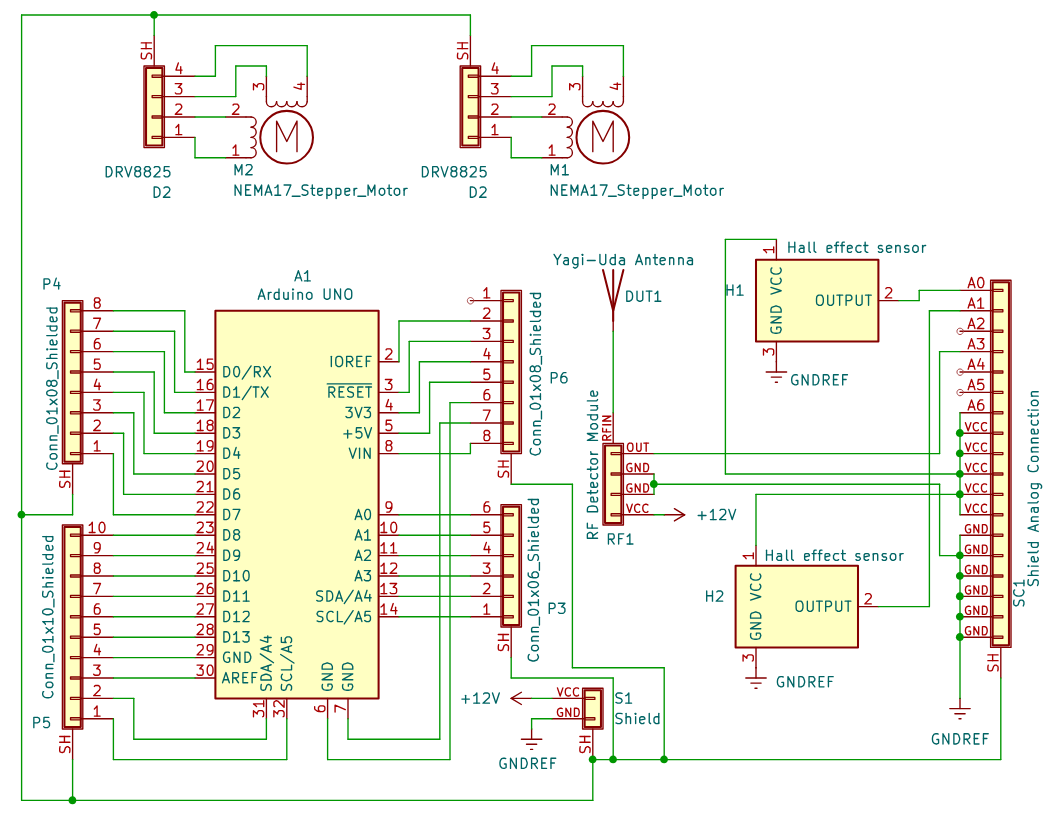
\includegraphics[width=0.7\textwidth]{Imagens/esquematico_ligacao.png}
    \caption{Detailed electrical schematic of the measurement system, illustrating component interconnections and pin assignments.}
    \label{cap3:sec3:fig1}
\end{figure}
\endgroup

\vspace{-0.1\baselineskip}

\indent Auxiliary components, such as the Hall-effect magnetic position sensors and the RF power detector module, connect to specific analog input pins provided by the shield. Sensor 1 is connected to analog pin A0, and Sensor 2 to analog pin A1. The AD8313 RF power module's analog output is connected to analog pin A3 of the shield, allowing the Arduino Uno to read the converted RF power signal.\\
\vspace{0.1cm}
Power distribution is managed centrally by the shield. An external 12V DC power supply provides the primary input to the shield. From this input, the shield directly supplies 12~V to both the stepper motors (via the DRV8825 drivers) and the AD8313 RF power module. Additionally, the shield incorporates an onboard voltage regulator that steps down the 12~V input to provide a stable 5~V supply, which powers the Arduino Uno board itself and the Hall-effect sensors. This integrated power management simplifies the wiring and ensures proper voltage levels for all components.\\
\vspace{0.1cm}
The shield also provides 5~V or 12~V output, depending on the physical configuration. In addition to the analog pins, the shield has digital pins, which were not used in this project but may be decisive in different approaches.



%-----------------------------------------------------------------------------------------------------
\section{Software Development}
\label{sec:software_development}
%-----------------------------------------------------------------------------------------------------
The software for the antenna radiation pattern measurement system comprises two main modules: Firmware implemented on an Arduino board, for motor control and a data acquisition and visualisation module developed in MATLAB.

The MATLAB and Arduino interact through the UART (Universal Asynchronous Receiver-Transmitter) protocol, following a sequence that begins with MATLAB, which initiates the measurement process by sending the scan parameters such as angular resolution and rotation range. The Arduino then executes the commands, moving the stepper motors through their drivers, performing the homing function with the Hall-effect sensors, and coordinating the acquisition of RF power values from the detector module. As the platform rotates stage by stage, the Arduino collects the corresponding measurements and transmits them back to MATLAB. In the meantime, MATLAB stores the data in a matrix, and after all measurements, the radiation pattern is plotted. This command $\rightarrow$ execution $\rightarrow$ response loop gives synchronisation between mechanical actuation and signal acquisition, helping in the measurement results.

The Arduino module controls the stepper motors, also performing a homing procedure to align the antenna to a $0 ^ \circ$ reference point. This reference detection is achieved by Hall-effect sensors. Rotations is carried out in increments (e.g., $1 ^ \circ$) according to commands received from MATLAB. Status confirmations are sent back via UART to ensure synchronisation. 

The MATLAB script communicates with the Arduino via a virtual communication (COM) port, employing the built-in \textit{serialport()} interface of MATLAB. The MATLAB function acquires RF signal data from the RF Module and stores it in a data matrix. It processes parameters such as directivity and generates polar plots (2D/3D) to visualise the antenna radiation pattern. 

The UART communication, established over a USB (Universal Serial Bus) connection, follows a command-response pattern, with MATLAB acting as the master and the Arduino as the slave. MATLAB sends rotation commands, and the Arduino returns measured power data in dBm. The data flow, illustrated in Figure~\ref{cap3:sec4:fig1}, begins with configuration in MATLAB, followed by command transmission, platform rotation, signal measurement, data storage, processing, and visualisation. 




\begin{figure}[H]
    \centering
    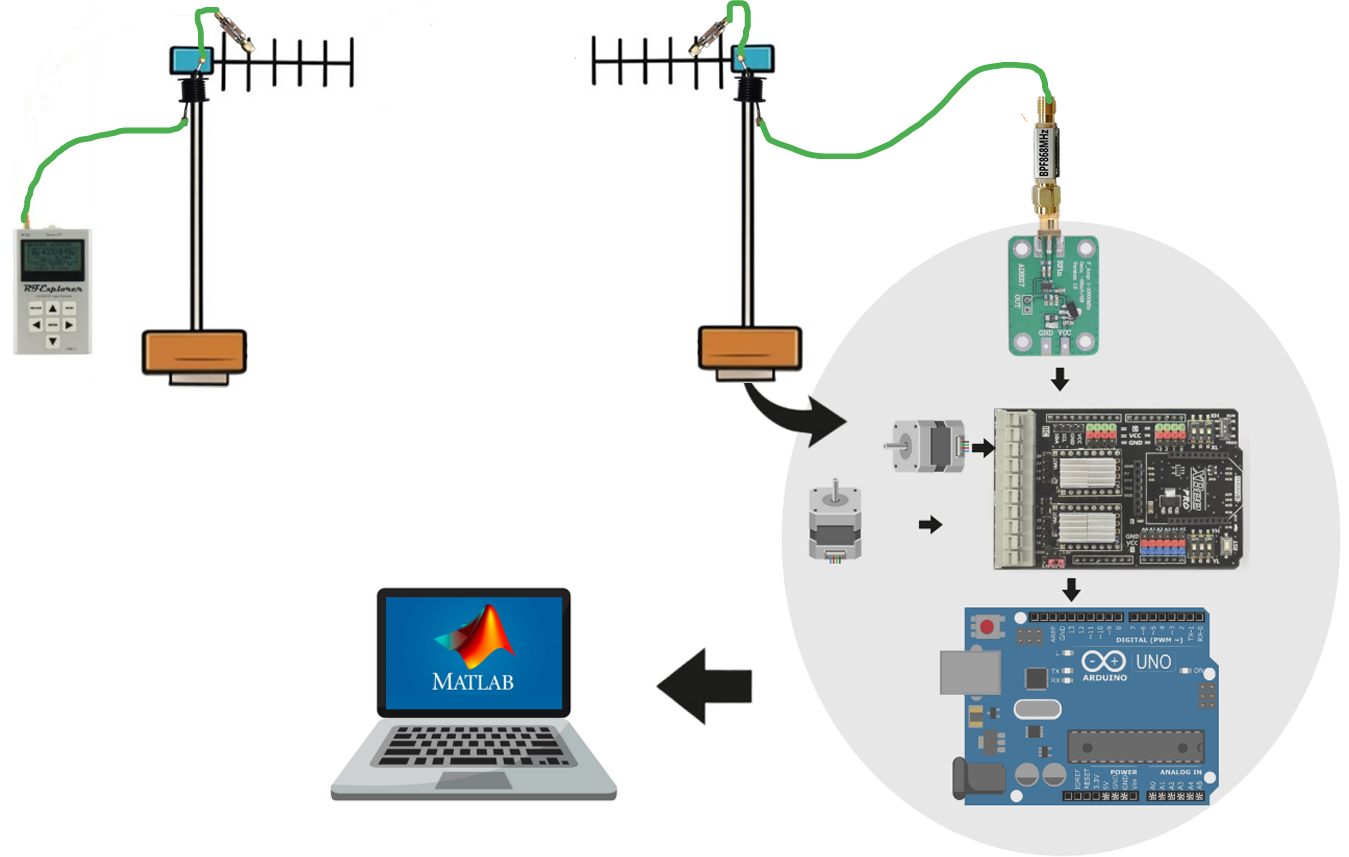
\includegraphics[width=0.9\textwidth]{Imagens/hardware_schematic.png}
    \caption{Schematic showing the flow of the signal from generation to analysis.}
    \label{cap3:sec4:fig1}
\end{figure}



%-----------------------------------------------------------------------------------------------------
\section{Validation Strategy}
\label{sec:validation_strategy}
%-----------------------------------------------------------------------------------------------------

To confirm the accuracy and reliability of the system, a series of validation tests were conducted following a structured testing protocol. This protocol began with characterisation of the transmitting and receiving antennas, as well as the bandpass filter, using a nanoVNA at 868 MHz in the ISM band. The filter, centred at 868 MHz with a bandwidth of 10 MHz, was selected for its ability to mitigate noise, though it introduced approximately 3 dB insertion loss attenuation. A linear model for signal power conversion was derived from the characterisation of the module, aligning closely with the datasheet specifications of the manufacturer.

The measurements were performed in an open environment to minimise unwanted reflections, as indoor settings would introduce excessive interference. In an ideal scenario, tests would be carried out in vacuum or an anechoic chamber, but, due to practical constraints, an outdoor setup was employed with consistent conditions across all trials. The radiation pattern was measured across azimuth angles ($0 ^ \circ$ to $360 ^ \circ$, $5 ^ \circ$ resolution), with 100 samples were averaged at each angle to reduce noise. To minimise cumulative angular errors and prevent cable entanglement (as wires were routed through tubes), measurements were performed bidirectionally: the platform rotated $180 ^ \circ$ in one direction, returned to the initial position, and then rotated $180 ^ \circ$ in the opposite direction. Ten measurement cycles were carried out to assess repeatability, with the averages plotted to verify consistency. The experimental results were compared with CST Studio Suite\footnote{The free educational version of this software was used in the simulations.} simulations, showing patterns that were closely aligned with those expected in the literature.\\
\vspace{0.1em}
\indent Antenna oscillation during rotation presented a challenge, resolved by increasing the pulley size on the stepper motor to enhance torque, enabling slower and more precise movements at the expense of measurement speed. The software was verified through command window messages in MATLAB and the Arduino IDE (Integrated Development Environment) to confirm reliable communication without errors.\\
\vspace{0.1em}
\indent The system supports other antennas, though only the Yagi-Uda was considered due to its richer characteristic radiation pattern. The validation, whose results will be provided in the next section, demonstrated that the system provides reliable and repeatable measurements, with limitations such as supported antenna size and reduced measurement speed for greater precision and reduced DUT (Device Under Test) oscillation. It therefore represents a cost-effective alternative to expensive commercial equipment for educational antenna studies.

%-----------------------------------------------------------------------------------------------------
\section{Development and Construction of the Yagi-Uda Antenna}
%-----------------------------------------------------------------------------------------------------

The Yagi-Uda antenna, first proposed by Shintaro Uda and popularised by Hidetsugu Yagi in 1926, is a directional antenna widely used for its high gain, relatively simple construction, and well-understood behaviour\cite{yagi1926}. Nearly a century after its conception, it remains a popular choice in applications ranging from broadcasting and amateur radio to modern wireless systems.

The operating frequency selected for the present project was 868 MHz, which lies within the ISM band allocated for licence-free operation in Europe \cite{etsi300220}. Although other ISM bands such as 433\,MHz could be used, the physical size of a half-wavelength element is inversely proportional to the frequency \cite{balanis2016}. Consequently, an antenna for 433\,MHz would be almost twice as large, making it impractical for the intended application. On the other hand, for frequencies above 1\,GHz, the resulting antenna would become very small, which could compromise mechanical robustness and ease of construction. Thus, the 868\,MHz frequency was chosen as an appropriate trade off between electrical performance and mechanical feasibility.

The Yagi-Uda antenna consists of a driven element (typically a half-wavelength dipole), a reflector placed behind it, which can take different configurations such as wire-grid, solid-plane, or curved-surface designs, and one or more directors positioned in front. In this work, a simple linear reflector was selected for its compatibility with the target frequency and ease of construction \cite{balanis2016, pozar2011}. The theoretical length $L$ of a half-wave element in free space is expressed as:
\begin{equation}
L \approx \frac{\lambda}{2} = \frac{c}{2 f}
\end{equation}
where $c$ is the speed of light in vacuum ($3 \times 10^{8}$\,m/s), $f$ is the operating frequency, and $\lambda$ is the wavelength. For $f = 868$\,MHz, $\lambda \approx 0.345$\,m and $L \approx 0.1725$\,m (172.5\,mm) before end-effect corrections.\\

However, in practice, due to the finite diameter of the elements and end effects, these ideal values require slight adjustments. Practical designs apply correction factors depending on the element diameter. Typical dimensions are \cite{balanis2016}:
\begin{align}
L_\text{reflector} &\approx (1.03 \pm 0.01) \times \frac{\lambda}{2} \\
L_\text{driven} &\approx (0.98 \pm 0.01) \times \frac{\lambda}{2} \\
L_\text{director} &\approx (0.95 \pm 0.01) \times \frac{\lambda}{2}
\end{align}
The spacing $S$ between elements is usually expressed as a fraction of the wavelength:
\begin{equation}
0.1\lambda \lesssim S \lesssim 0.25\lambda
\end{equation}
\vspace{-0.1em}
\indent When the reflector is placed closer to the driven element, the front-to-back ratio increases, but impedance matching may degrade. In contrast, increasing reflector spacing can broaden bandwidth at the expense of front-to-back performance. For directors, reducing spacing increases gain up to a point, but excessive closeness can raise mutual coupling and narrow bandwidth. Larger director spacing reduces coupling, but may decrease gain and introduce sidelobes. Figure~\ref{cap3:sec6:fig1} shows the simulated antenna in CST Studio Suite.
\vspace{-0.1em}\\
\indent It should be noted that the mechanical support structure, namely the boom, fabricated in PLA during the construction stage, was not represented in the simulation model. This omission is justified since PLA exhibits a relative permittivity of approximately $2.7-2.9$ and a relative permeability close to $1$, which makes it effectively transparent to RF radiation \cite{8323386}. As a result, including the boom in the CST model would not significantly affect the simulated radiation pattern or input impedance. The physical implementation of the PLA boom and its role in the antenna assembly will be detailed in the subsequent section.


\begin{figure}[H]
\centering
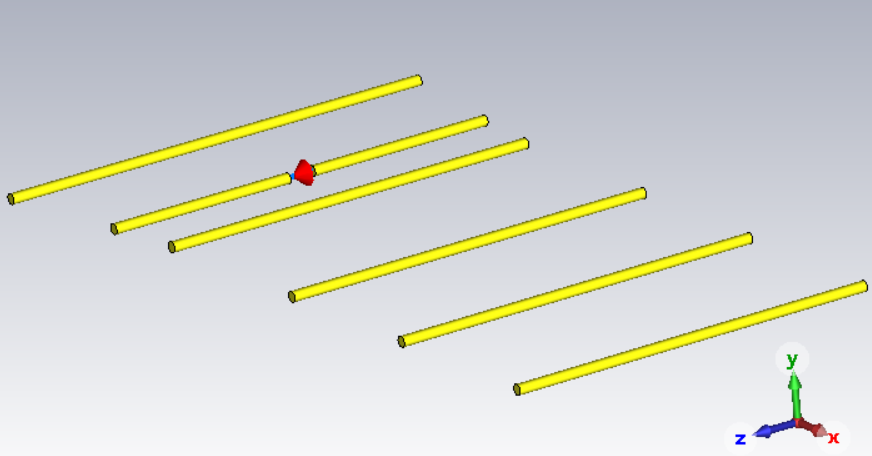
\includegraphics[width=0.9\linewidth]{Imagens/CST_Antenna.png}
\caption{Yagi-Uda antenna simulated in CST Studio Suite.}
\label{cap3:sec6:fig1}
\end{figure}

\subsection{Simulation and Dimensions}

The optimised element lengths and spacings obtained in CST Studio Suite are given in Table~\ref{cap3:sec6:table1}\protect\footnotemark\footnotetext{The reference position is measured from the midpoint between the two halves of the driven dipole element. The boom is aligned with the central axis of the elements.}, and the constructed prototype is shown in Figure~\ref{cap3:sec6:fig2: b}. 
Two identical Yagi-Uda antennas were constructed based on these specified dimensions: one dedicated to transmission and the other to reception. This configuration enabled testing the antenna performance within a representative communication link scenario.


\begin{table}[H]
\centering
\caption{Element lengths and spacings for the Yagi-Uda antenna.}
\label{cap3:sec6:table1}
\begin{tabular}{lcc}
\hline
Element & Length (mm) & Position (mm) \\
\hline
Reflector & 166.41 & -51.964 \\
Driven & 150.98 & 0.0 \\
Director 1 & 143.85 & 30.104 \\
Director 2 & 142.16 & 102.131 \\
Director 3 & 140.48 & 166.814 \\
Director 4 & 139.51 & 234.902 \\
\hline
\end{tabular}
\end{table}


\subsection{Building the Yagi-Uda Antenna}
\label{cap3:sec6:subsec2:build_antenna}

The antenna was modelled mechanically in SolidWorks\footnote{Educational version licensed to the Polytechnic Institute of Bragança.} (Figure~\ref{cap3:sec6:fig2: a}) and the boom was fabricated using fused deposition modelling (FDM) with PLA, as shown in Figure \ref{cap3:sec6:fig2: b}. The radiating elements were made from solid brass rods with a diameter of 3\,mm\footnote{Brass composition was approximately two-thirds copper and one-third zinc.}. %, with conductivity $\sigma = 15.9 \times 10^{6}$\,S/m and thickness $d = 0.68 \times 10^{-3}$\,m.%



\begin{figure}[H]
     \centering
     \begin{subfigure}{0.552\textwidth}
         \centering
         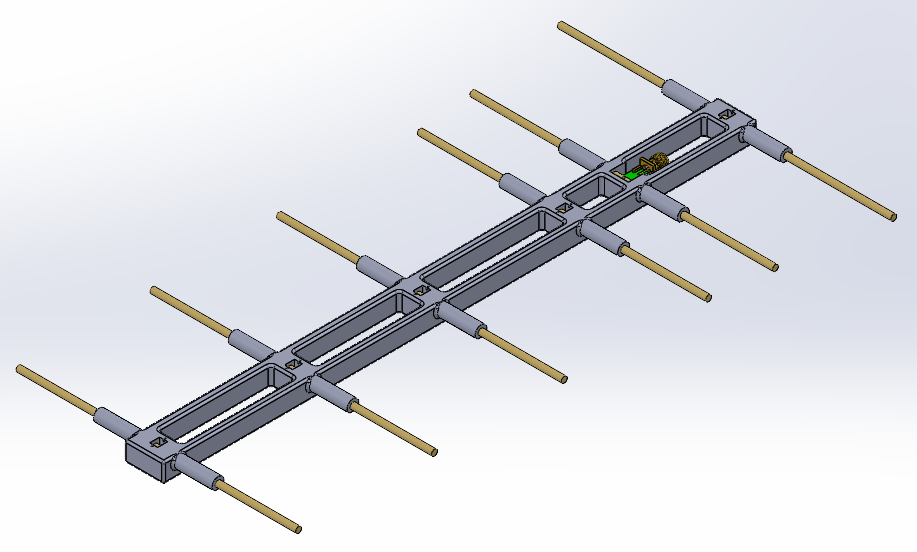
\includegraphics[width=\textwidth]{Imagens/Solidworks_antena.png}
         \caption{Mechanical model in SolidWorks}
         \label{cap3:sec6:fig2: a}
     \end{subfigure}
     \hspace{1mm}
     \begin{subfigure}{0.405\textwidth}
         \centering
         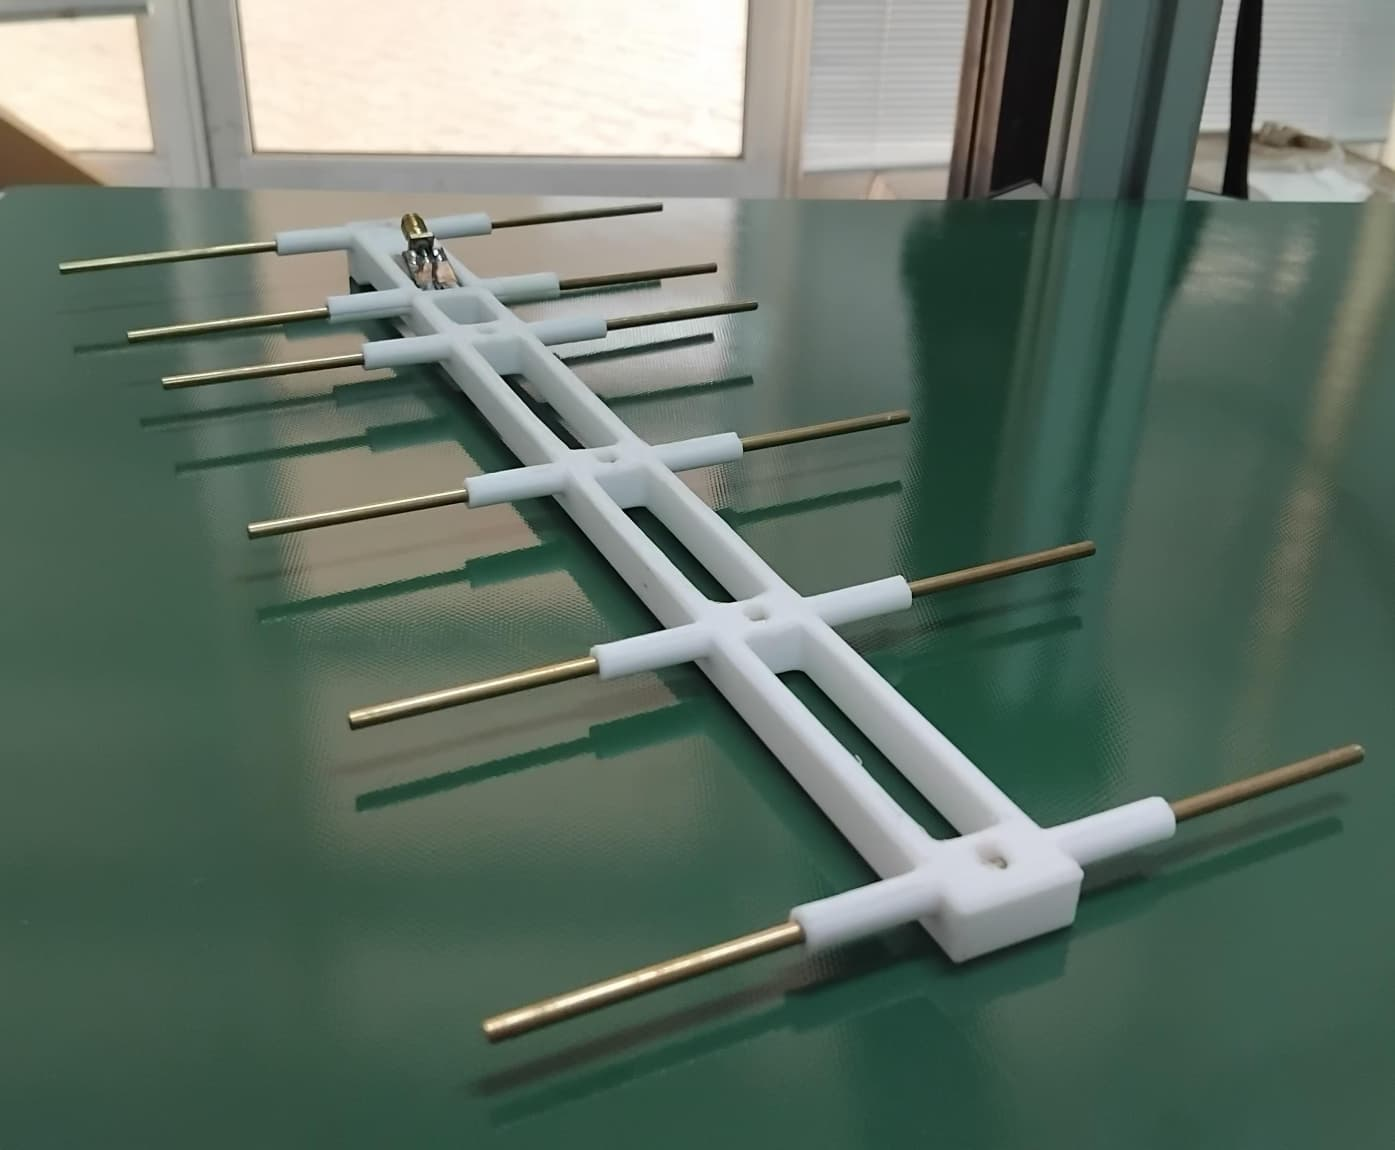
\includegraphics[width=\textwidth]{Imagens/antenna_prototype.jpeg}
         \caption{Constructed prototype}
         \label{cap3:sec6:fig2: b}
     \end{subfigure}
        \caption{Mechanical model of the antenna developed in SolidWorks and the constructed Yagi-Uda antenna prototype.}
        \label{cap3:sec6:fig2}
\end{figure}


%-----------------------------------------------------------------------------------------------------
\subsection{Antenna Characterisation}
\label{cap3:sec6:subsec3}
%-----------------------------------------------------------------------------------------------------

The reflection coefficient $S_{11}$ and the VSWR of the transmitting and receiving antennas were measured with the NanoVNA. both antennas exhibited nearly identical responses, as expected from their close design, with only minor construction tolerances causing negligible deviations; therefore, only one set of results is presented in Figure~\ref{cap3:sec6:subsec3:fig1} for conciseness. Minor variations between them are expected due to construction tolerances, but no significant deviations were observed.

The resonance occurs close to the intended frequency of 868~MHz. The optimum impedance matching condition was obtained at approximately 876~MHz, where $S_{11}$ reached around $-13$~dB and the VSWR was 1.58. At 868~MHz, the measured values were $S_{11} \approx -11$~dB and VSWR $\approx 1.77$, corresponding to an input impedance of about $30 + j0.7~\Omega$. The $-10$~dB bandwidth extends from 865~MHz to 890~MHz, resulting in approximately 25~MHz, which is consistent across both NanoVNA and QucsStudio measurements.

\begin{figure}[H]
    \centering
    \begin{subfigure}{0.99\textwidth}
        \centering
        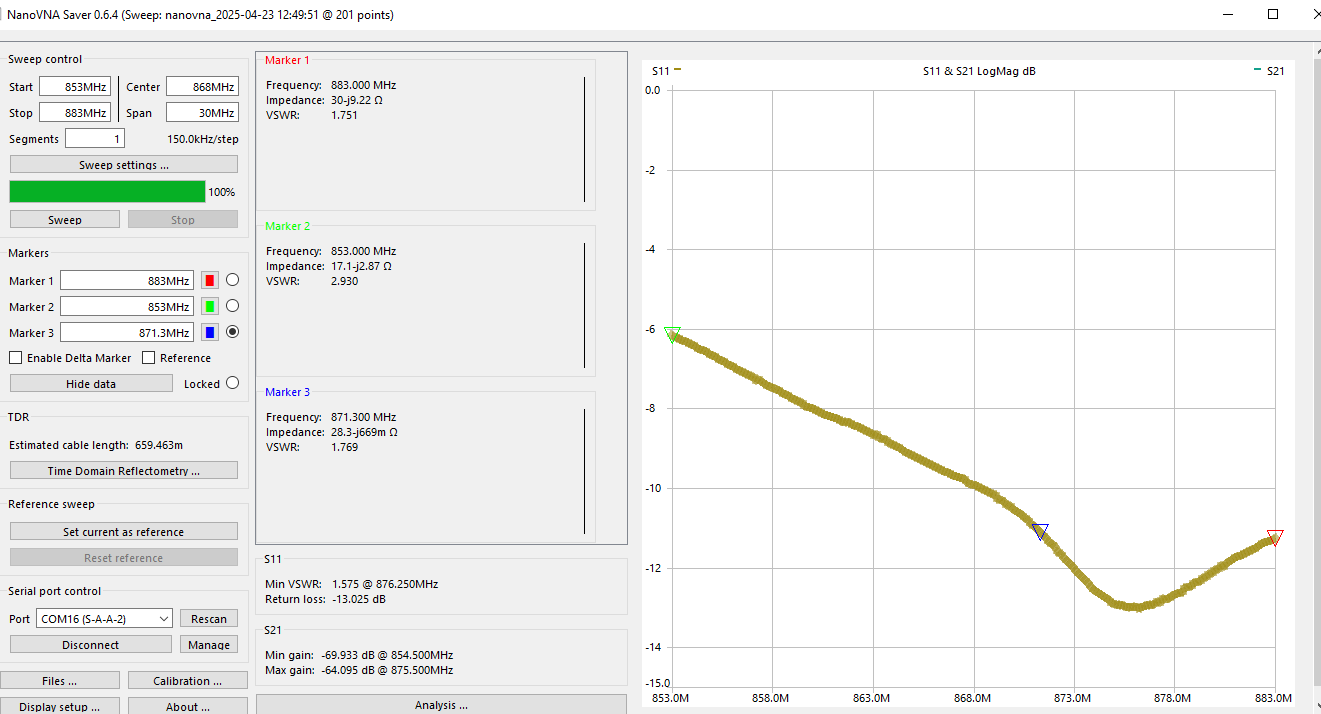
\includegraphics[width=\textwidth]{Imagens/Antena Transmissora/Caraterização VNA/Fig2.png}
        \caption{$S_{11}$}
        \label{cap3:sec6:subsec3:fig1:a}
    \end{subfigure}
    \hfill
    \begin{subfigure}{0.99\textwidth}
        \centering
        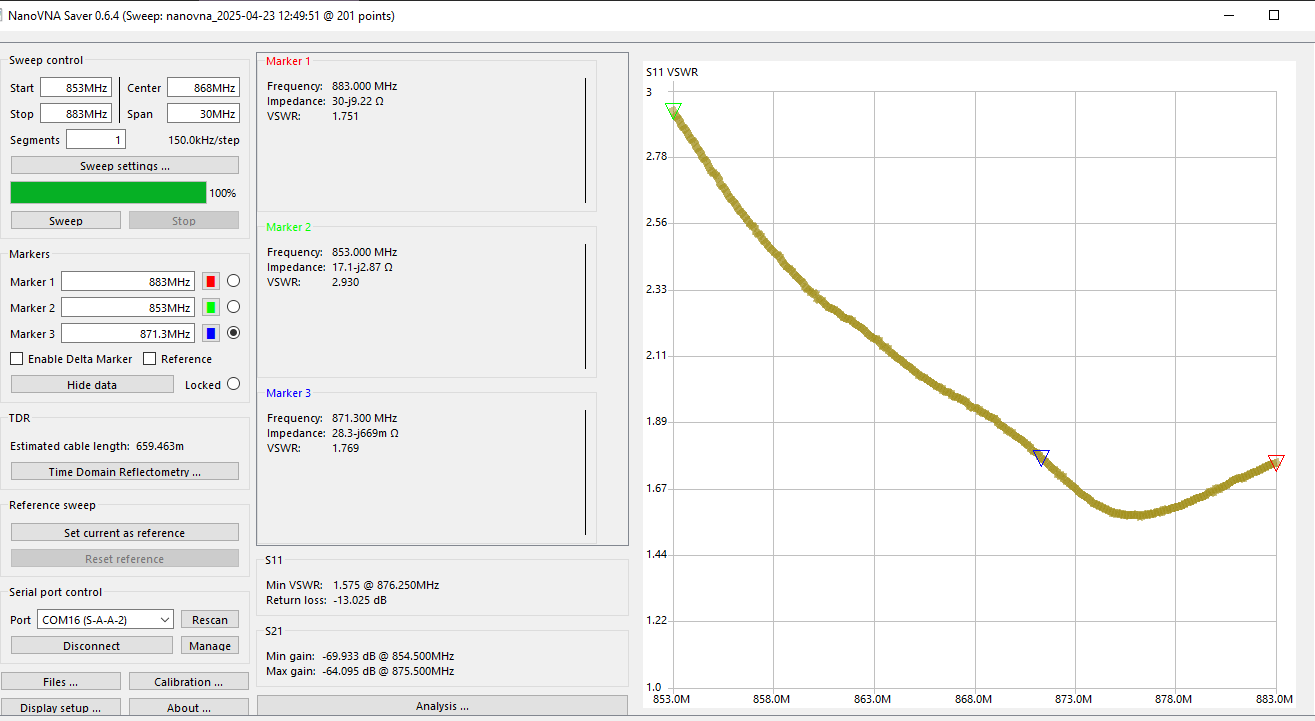
\includegraphics[width=\textwidth]{Imagens/Antena Transmissora/Caraterização VNA/Fig4.png}
        \caption{VSWR}
        \label{cap3:sec6:subsec3:fig1:b}
    \end{subfigure}
    \caption{Characterisation of the antenna using the NanoVNA.}
    \label{cap3:sec6:subsec3:fig1}
\end{figure}

Overall, the antennas demonstrate acceptable matching around the ISM band, validating their suitability for the subsequent radiation pattern measurements. Nevertheless, clearly could be better parameters.

%-----------------------------------------------------------------------------------------------------
\section{RF Signal Integrity: Balun and Impedance Matching Network}
\label{sec:Balun_Impedance-matching}
%-----------------------------------------------------------------------------------------------------

In RF systems, optimal power transfer and signal integrity depend not only on the antenna geometry but also on suppressing undesired current modes and ensuring accurate impedance matching between interconnected components \cite{balanis2016}. Since the nominal characteristic impedance of most RF systems is $50,\Omega$, particular attention was given to this requirement during the antenna design.

Therefore, two strategies were  implemented: (i) mitigation of common-mode currents through the use of a balun, and (ii) the design of an impedance matching network to ensure a $50\,\Omega$ interface between the antenna and the transmission line, as well the RF sensor module.

\subsection{Balun for Common-Mode Current Suppression}

When a balanced antenna, such as the Yagi-Uda, is connected to an unbalanced coaxial transmission line, common-mode currents can propagate along the shield of the coaxial cable. These currents can cause radiation from the feed line itself, altering the antenna radiation pattern and impedance characteristics \cite{Fiorelli2011,Icheln2004}. To mitigate this effect, a current balun was implemented, functioning as a choke to suppress common-mode currents without affecting the desired differential-mode signal \cite{Duffy2022, Sevick2001}.

The balun geometry was designed using analytical calculations that considered the type of coaxial cable (RG-174) and its physical dimensions, as the conductor diameter and dielectric properties directly influence the inductance, the skin effect, and the ability to suppress common-mode currents at RF. A MATLAB script was used to determine the optimal number of turns and winding diameter for operation at the target frequency\footnote{The MATLAB script in Appendix~\ref{apendice5} was used for the geometric design of the balun.}.\\
\vspace{0.1em}
\indent The design and evaluation stages included both simulation and measurement. After confirming through VNA measurements, as seen in Figure \ref{fig:balun_fotos_all}, that the geometry provided effective suppression, the balun was manufactured as illustrated in Figure~\ref{cap3:sec7:fig1}.

\begin{figure}[H]
    \centering
    % Esquerda: imagem grande
    \begin{subfigure}[b]{0.482\textwidth}
        \centering
        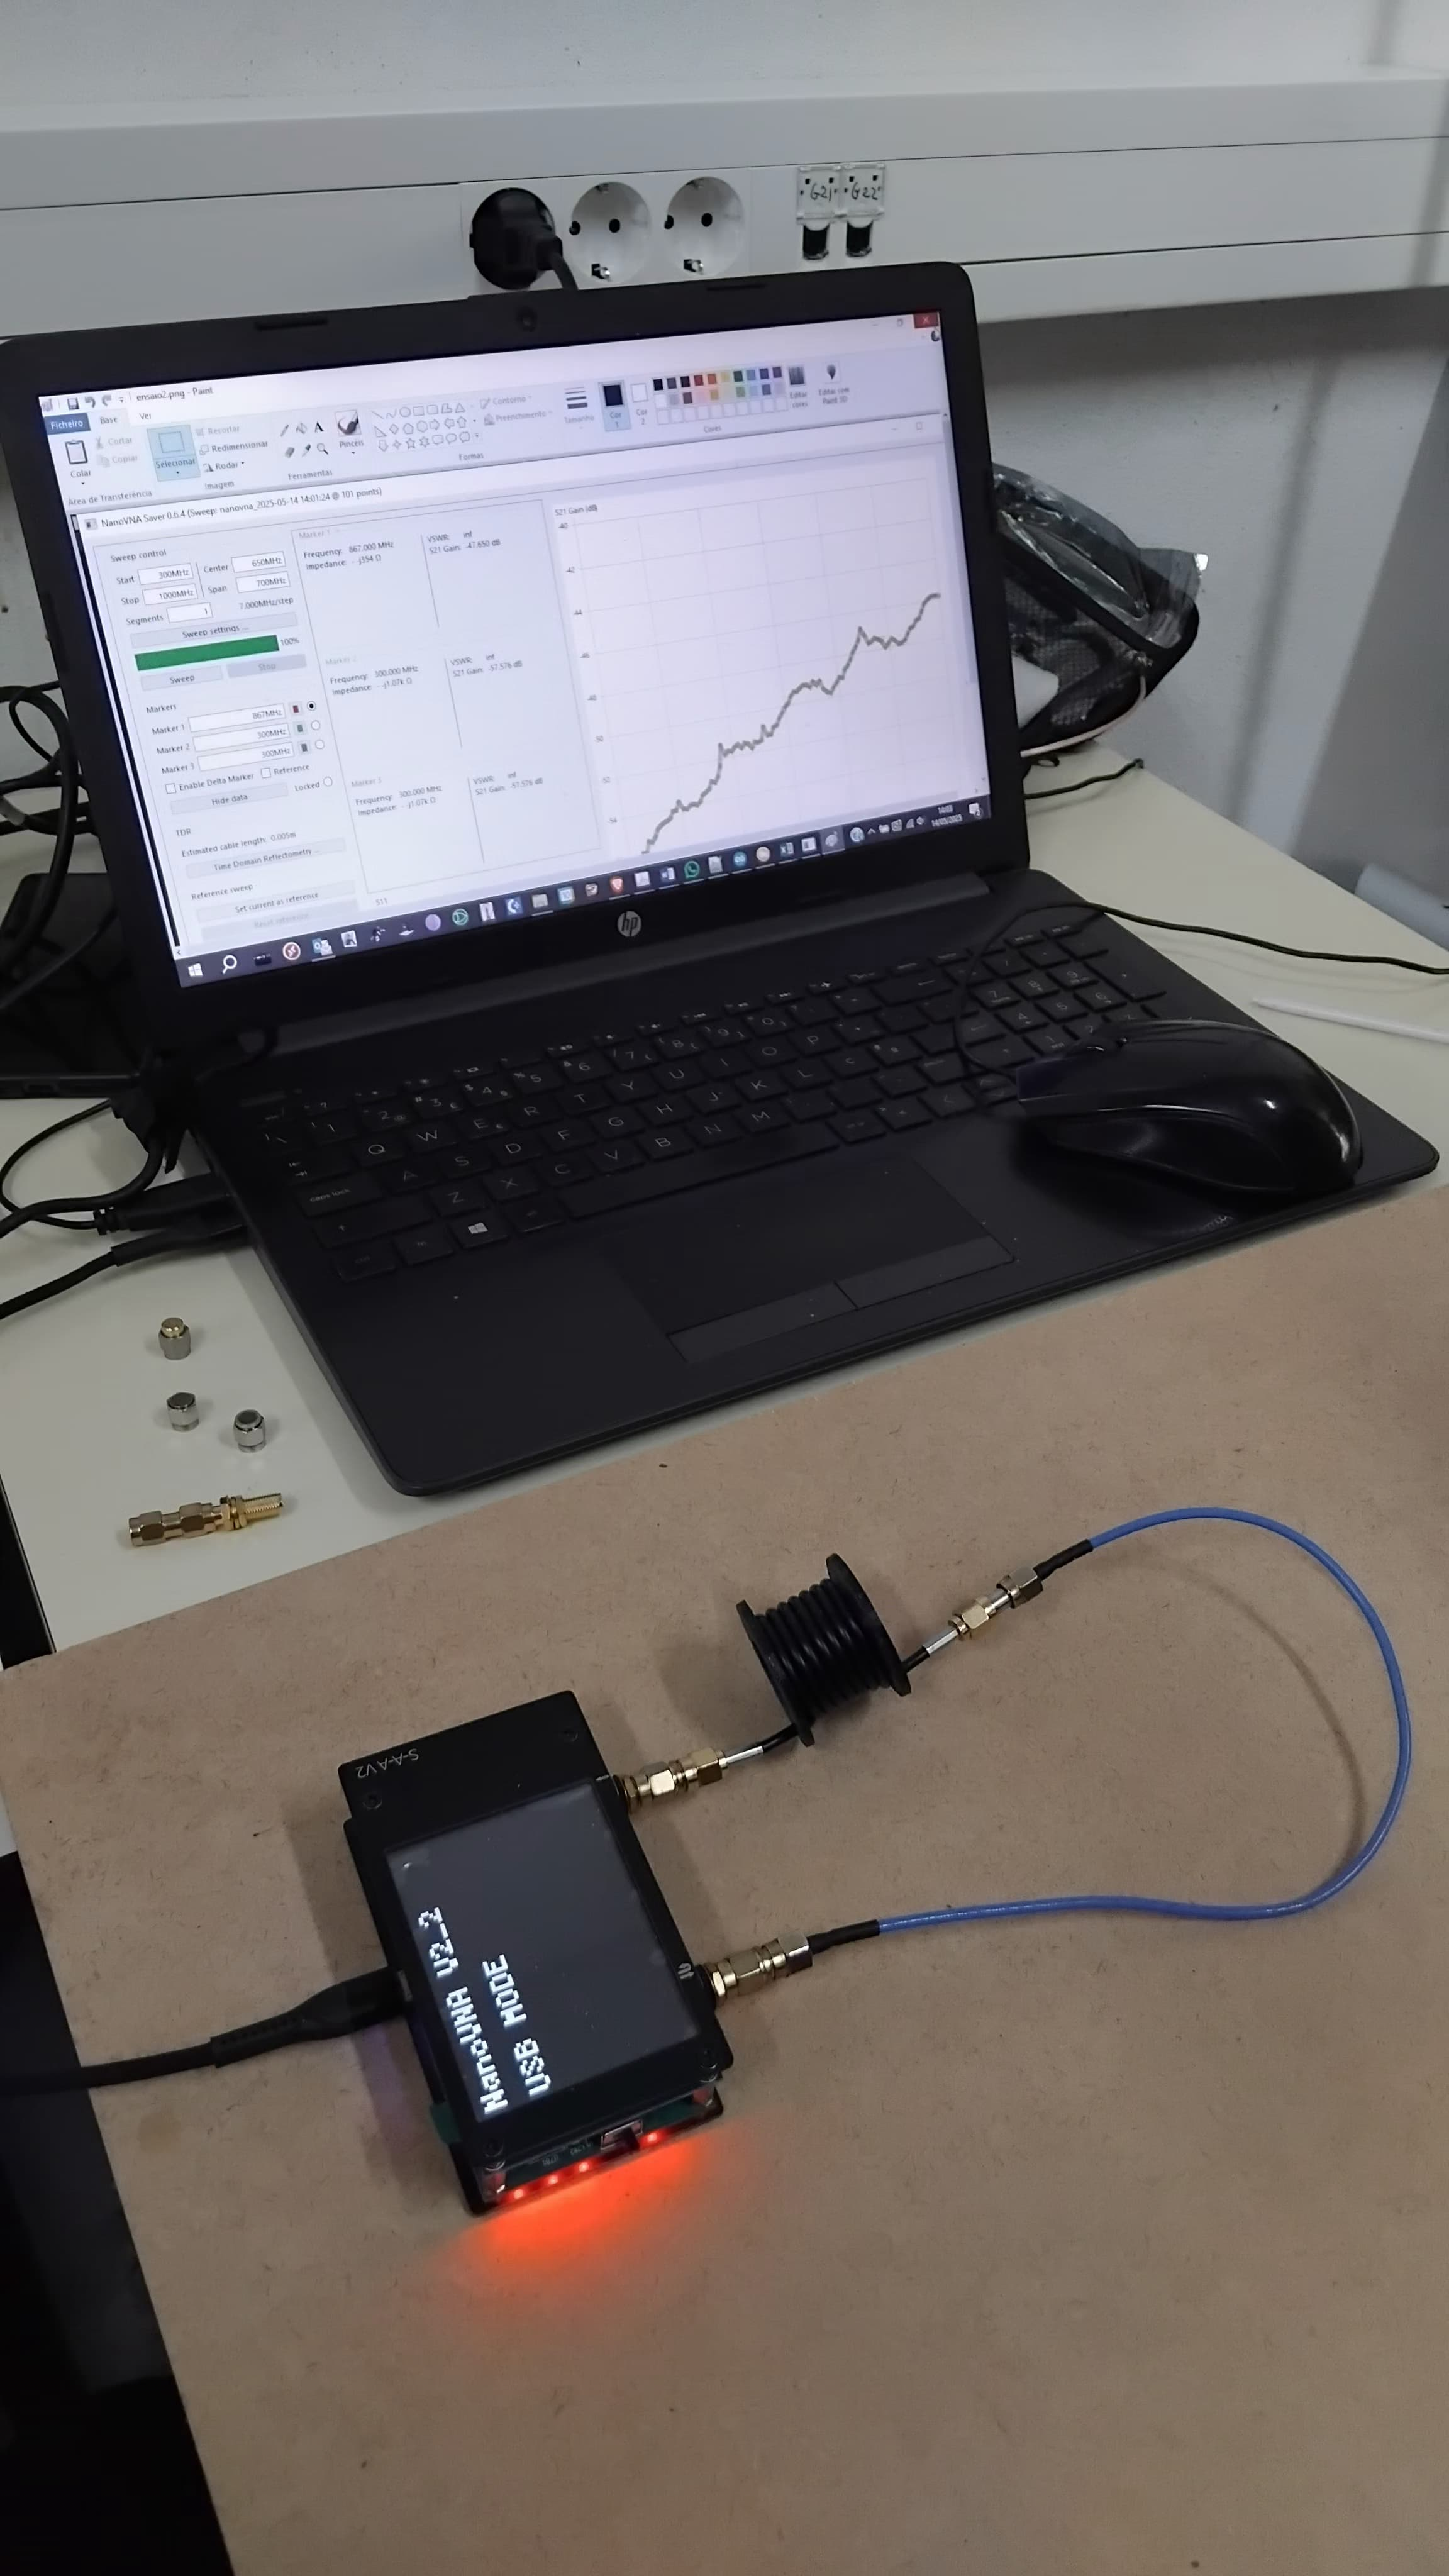
\includegraphics[width=\textwidth]{Imagens/balun3.jpg}
        \caption{Balun during characterisation.}
        \label{fig:balun_foto_lateral}
    \end{subfigure}
    \hspace{2mm}
    % Direita: duas imagens menores empilhadas
    \begin{subfigure}[b]{0.48\textwidth}
        \centering
        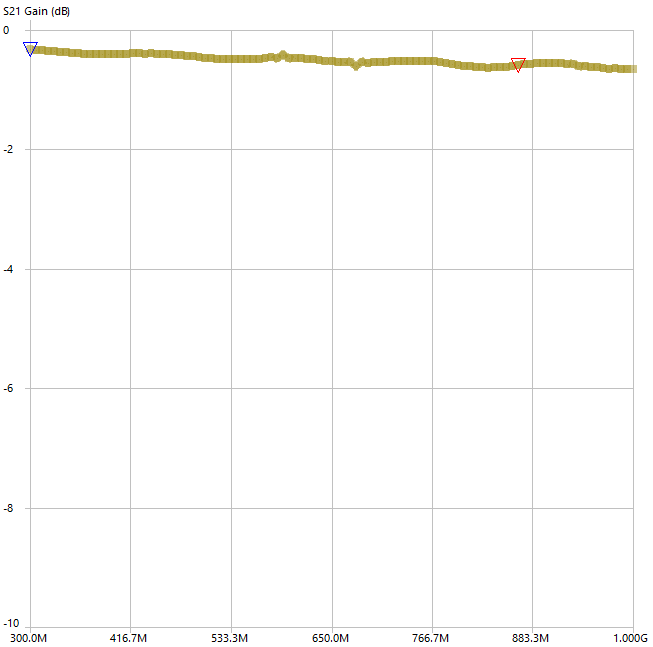
\includegraphics[width=0.845\textwidth]{Imagens/balun_caract/insertion_loss.png}
        \caption{Differential mode.}
        \label{fig:balun_foto_regua}
        \vskip 2mm
        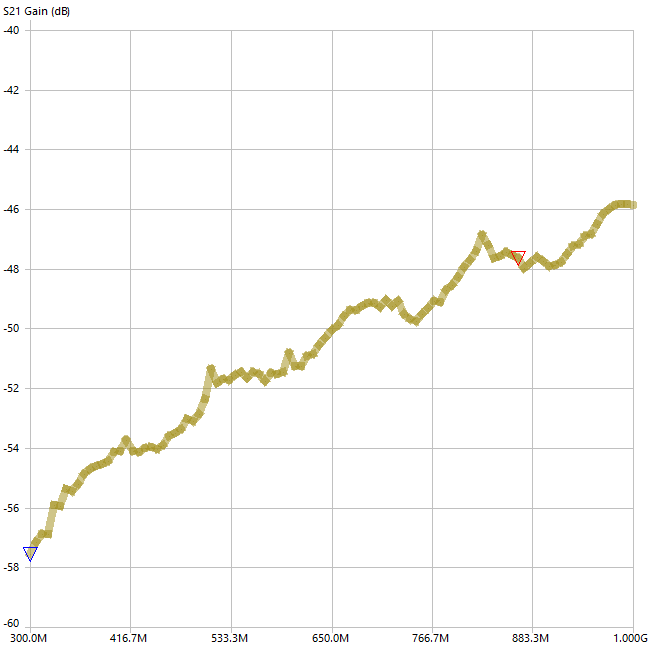
\includegraphics[width=0.845\textwidth]{Imagens/balun_caract/insertion_loss2.png}
        \caption{Common mode.}
        \label{fig:balun_foto_superior}
    \end{subfigure}
    \caption{Characterisation of the air choke balun.}
    \label{fig:balun_fotos_all}
\end{figure}

\begin{figure}[H]
    \centering
    \begin{subfigure}{0.427\textwidth}
        \centering
        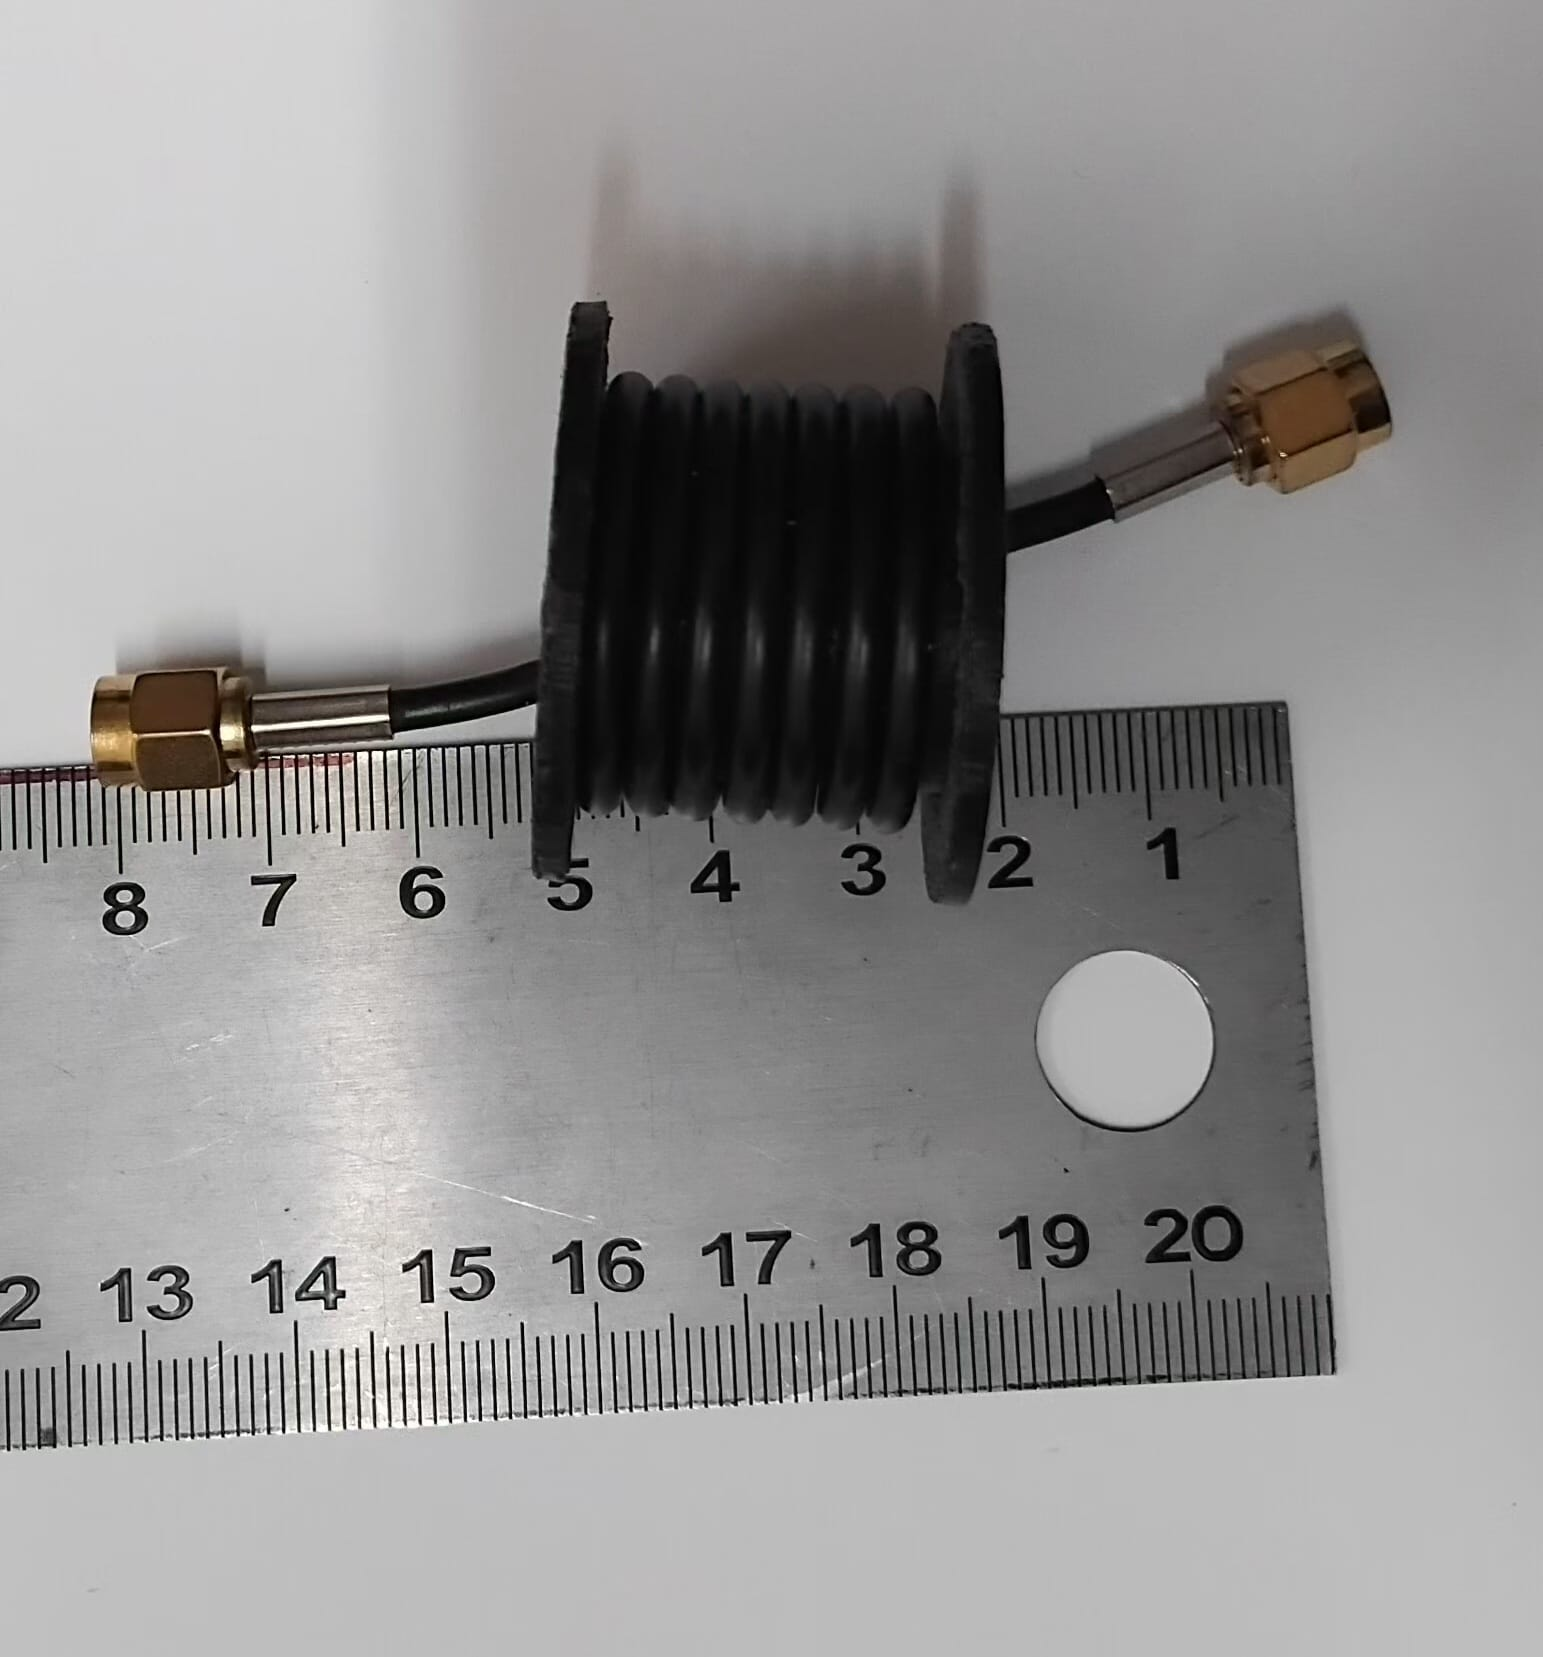
\includegraphics[width=\textwidth]{Imagens/balun.jpg}
        \caption{Balun and a measuring tape.}
        \label{cap3:sec7:fig1:a}
    \end{subfigure}
    \hspace{1mm}
    \begin{subfigure}{0.4875\textwidth}
        \centering
        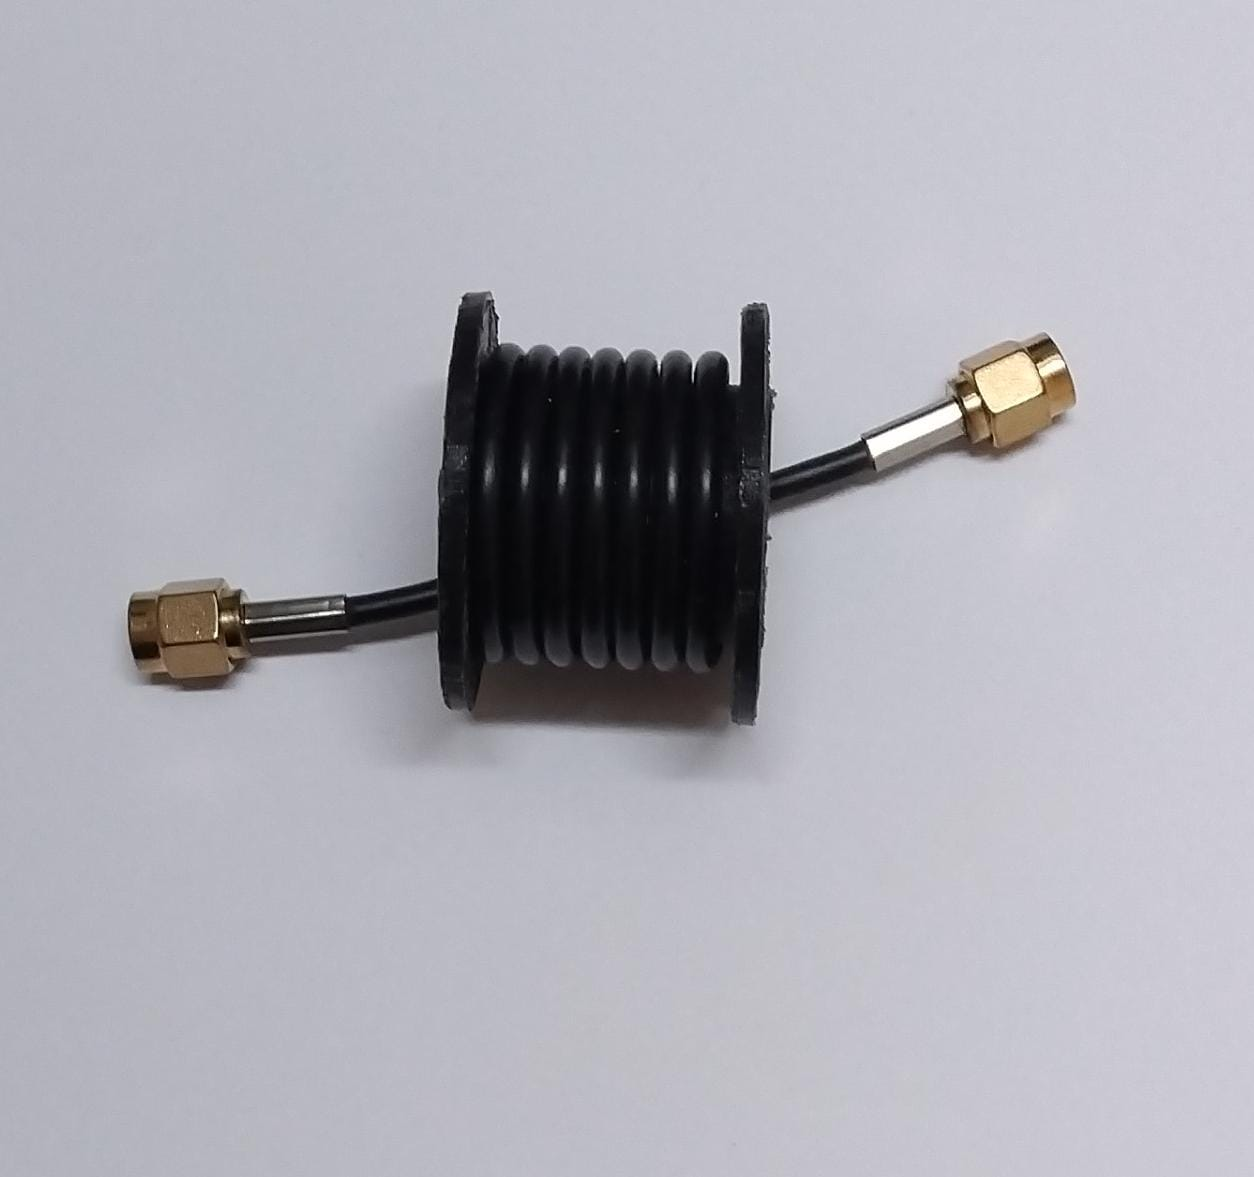
\includegraphics[width=\textwidth]{Imagens/balun2.jpg}
        \caption{Top view of the balun.}
        \label{cap3:sec7:fig1:b}
    \end{subfigure}
    \caption{Photos of the air choke balun manufactured using RG174 cable, with 3D printed support.}
    \label{cap3:sec7:fig1}
\end{figure}

%-----------------------------------------------------------------------------------------------
\subsection{Impedance Matching Network Design}
%-----------------------------------------------------------------------------------------------


After antenna characterisation, as seen in Subsection~\ref{cap3:sec6:subsec3}, it became evident that impedance matching was required due to the observed mismatch with the $50\,\Omega$ reference\cite{ARRL2023}. Initial estimates for the matching network components (capacitor and inductor) were obtained using QucsStudio and CST simulations, considering the antenna response alone. However, these values needed refinement once the effect of the PCB layout was included. For this reason, the PCB was first characterised in its bare form, without components, to quantify its intrinsic parasitic contributions.

The shunt PCB impedance, $|Z| \approx 21.5~\Omega$, was obtained from the measured $S_{21}$, as shown in Figure \ref{fig:pcb_s21_curve}. Then, the corresponding parasitic capacitance follows from Equation~\eqref{eq:capacitance_from_impedance}. This measurement yielded $C \approx 8.5~\text{pF}$. Simulations independent of the PCB (CST and QucsStudio) gave $C \approx 7.8~\text{pF}$, in close agreement with the experimental result. Figures \ref{fig:cst_results} and \ref{fig:qucs_results} show the models and results obtained from the simulations.


\begin{figure}[H]
    \centering
    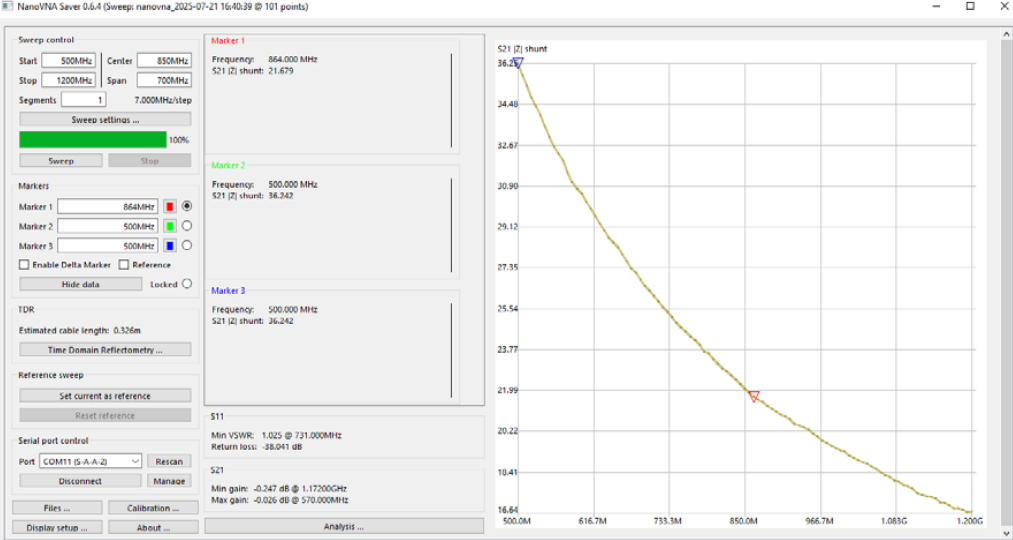
\includegraphics[width=0.75\linewidth]{Imagens/NanoVNA_PCB_S21.png}
    \caption{Measured $S_{21}$ curve of the bare PCB with NanoVNA Saver.}
    \label{fig:pcb_s21_curve}
\end{figure}


\begin{align}
C &= \frac{1}{2 \pi f |Z|} \label{eq:capacitance_from_impedance} = \frac{1}{2 \pi \cdot (868 \times 10^{6}) \cdot 21.5}
\approx 8.5~\text{pF}
\end{align}

\begin{figure}[H]
    \centering
    \begin{subfigure}{0.8\textwidth}
        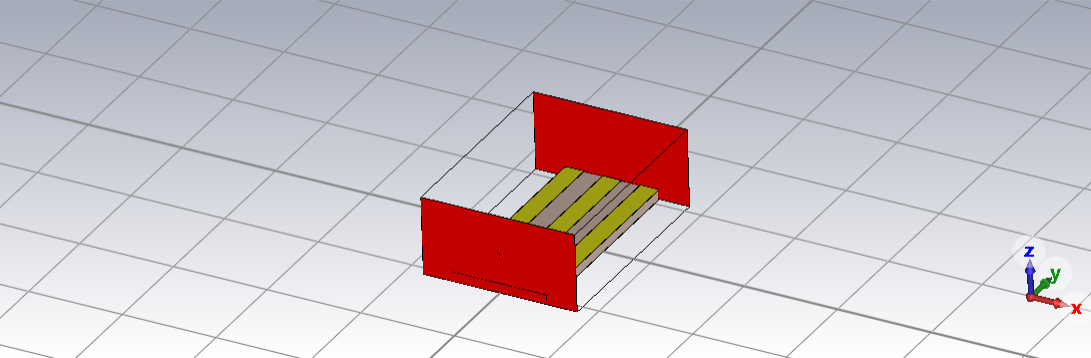
\includegraphics[width=\linewidth]{Imagens/CST_Model.png}
        \caption{CST PCB model}
        \label{fig:cst_model}
    \end{subfigure}\hfill
    \begin{subfigure}{0.8\textwidth}
        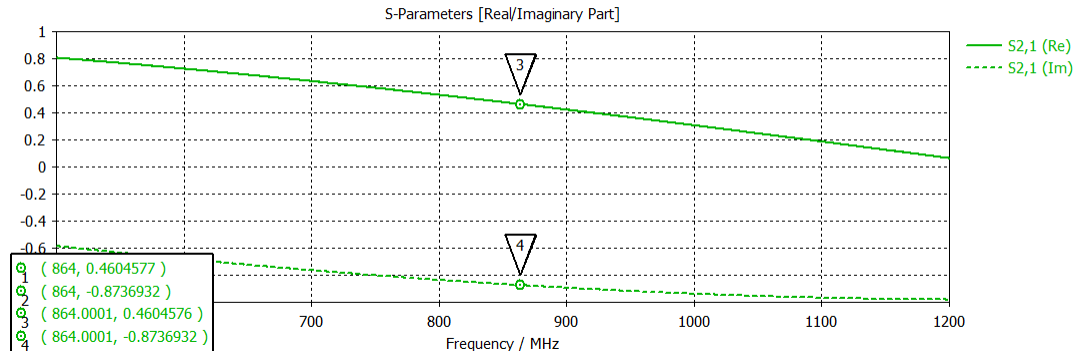
\includegraphics[width=\linewidth]{Imagens/CST_Results.png}
        \caption{CST simulation result}
        \label{fig:cst_resultb}
    \end{subfigure}
    \caption{CST Studio Suite simulation of the PCB}
    \label{fig:cst_results}
\end{figure}

\begin{figure}[H]
    \centering
    \begin{subfigure}{0.85\textwidth}
        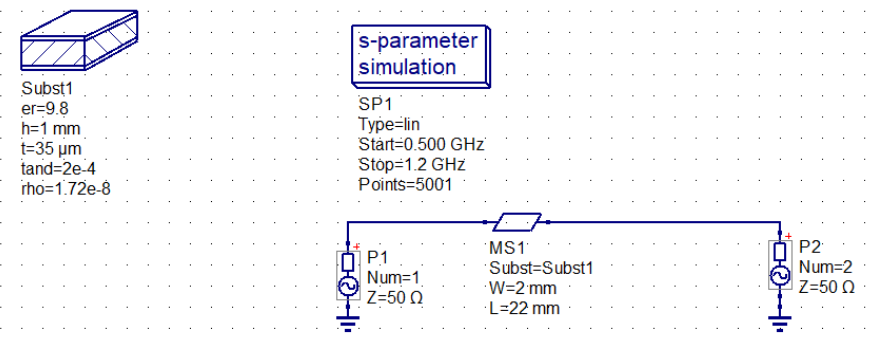
\includegraphics[width=\linewidth]{Imagens/Qucs_Model.png}
        \caption{QucsStudio PCB model}
        \label{fig:qucs_model}
    \end{subfigure}\hfill
    \begin{subfigure}{0.75\textwidth}
        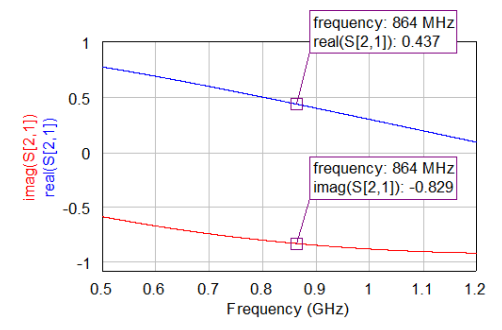
\includegraphics[width=\linewidth]{Imagens/Qucs_Results.png}
        \caption{QucsStudio simulation result}
        \label{fig:qucs_result}
    \end{subfigure}
    \caption{QucsStudio simulation of the PCB: (a) model and (b) result.}
    \label{fig:qucs_results}
\end{figure}

\begin{equation}
Z = Z_0 \cdot \frac{S_{21}}{2(1 - S_{21})}, \quad Z_0 = 50~\Omega
\label{eq:impedance_from_s21}
\end{equation}

\begin{equation}
Z_{\text{CST}} = 50 \cdot \frac{0.460458 - j0.873693}{2\left(1 - (0.460458 - j0.873693)\right)}
\approx -12.21 - j20.71~\Omega
\label{eq:Z_CST}
\end{equation}

\begin{equation}
|Z_{\text{CST}}| = \sqrt{(-12.21)^2 + (-20.71)^2} \approx 24.04~\Omega
\label{eq:Z_CST_module}
\end{equation}

\begin{align}
C_{\text{CST}} &= \frac{1}{2 \pi \cdot 864 \times 10^{6} \cdot 24.04} \label{eq:C_CST} \\
C_{\text{CST}}&\approx 7.66 \times 10^{-12}\ \text{F}\\
C_{\text{CST}}&= 7.66~\text{pF}
\end{align}

\begin{align}
Z_{\text{Qucs}} &= 50 \cdot \frac{0.437 - j0.829}{2\left(1 - (0.437 - j0.829)\right)} \label{eq:Z_QUCS} \\
Z_{\text{Qucs}}&\approx -10.98 - j20.64~\Omega
\end{align}

\begin{equation}
|Z_{\text{Qucs}}| = \sqrt{(-10.98)^2 + (-20.64)^2} \approx 23.38~\Omega
\label{eq:Z_QUCS_module}
\end{equation}

\begin{align}
C_{\text{Qucs}} &= \frac{1}{2 \pi \cdot 864 \times 10^{6} \cdot 23.38} \label{eq:C_QUCS} \\
C_{\text{Qucs}}&\approx 7.87 \times 10^{-12}\ \text{F} \\
C_{\text{Qucs}}&= 7.87~\text{pF}
\end{align}

\vspace{0.1em}
\indent As noted, the results of the measurements and simulations (CST and QucsStudio) are in close agreement, producing parasitic capacitance values in the range of $7.66$ to $8.5$ pF. This consistency confirms that the PCB introduces significant capacitance, which would be an issue if it was not considered for the impedance matching design\cite{Saario2003}.\\
\vspace{0.1em}
\indent After, all S-parameters were acquired to build a Touchstone file of the PCB for co-simulation with the DUT. With the NanoVNA, the sweep was performed to obtain $S_{11}$ and $S_{21}$, and the ports were inverted to acquired the $S_{22}$ and $S_{12}$. Then, they were merged into a single two-port file. The measured responses are shown in Figure~\ref{fig:pcb_full_sparams}, while the resulting files were validated in Qucs before use, is illustrated in Figure~\ref{fig:touchstone}.

\begin{figure}[H]
    \centering
    \begin{subfigure}{0.49\textwidth}
        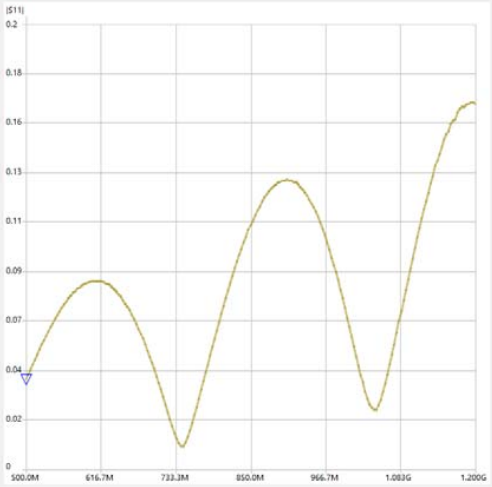
\includegraphics[width=\linewidth]{Imagens/NanoVNA_S11.png}
        \caption{Measured $S_{11}$}
        \label{fig:pcb_s11}
    \end{subfigure}
    \hfill
    \begin{subfigure}{0.49\textwidth}
        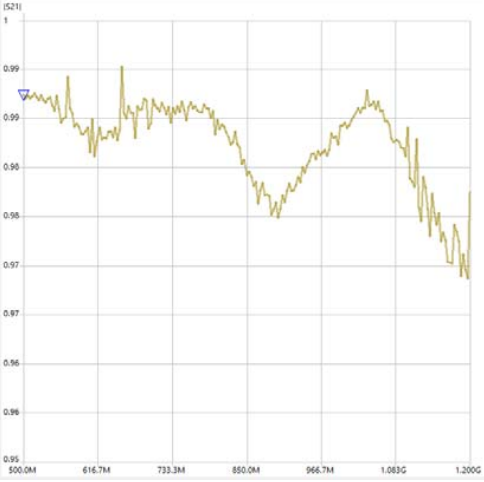
\includegraphics[width=\linewidth]{Imagens/NanoVNA_S21.png}
        \caption{Measured $S_{21}$}
        \label{fig:pcb_s21}
    \end{subfigure}
    \vskip 2mm
    \begin{subfigure}{0.49\textwidth}
        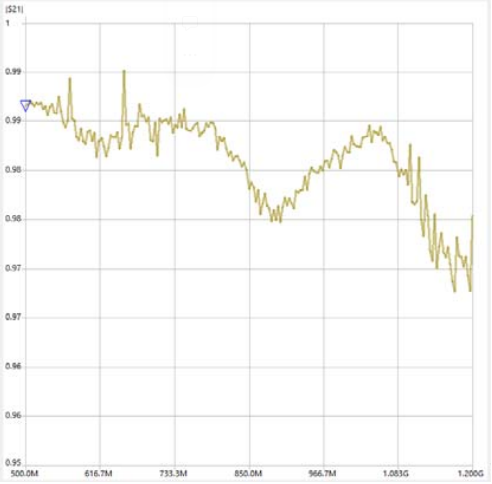
\includegraphics[width=\linewidth]{Imagens/NanoVNA_S12.png}
        \caption{Measured $S_{12}$}
        \label{fig:pcb_s12}
    \end{subfigure}
    \hfill
    \begin{subfigure}{0.49\textwidth}
        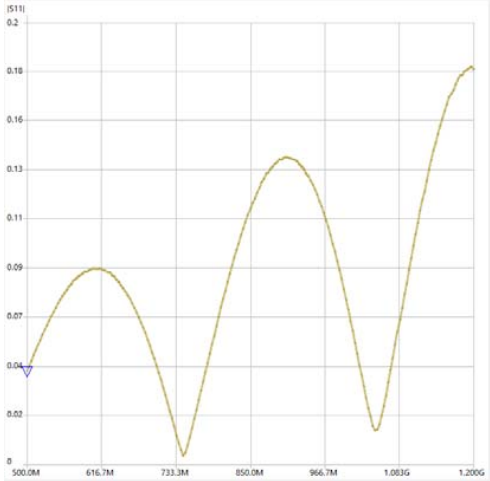
\includegraphics[width=\linewidth]{Imagens/NanoVNA_S22.png}
        \caption{Measured $S_{22}$}
        \label{fig:pcb_s22}
    \end{subfigure}
    \caption{Measured S-parameters of the PCB using NanoVNAsaver.}
    \label{fig:pcb_full_sparams}
\end{figure}



\begin{figure}[H]
    \centering
    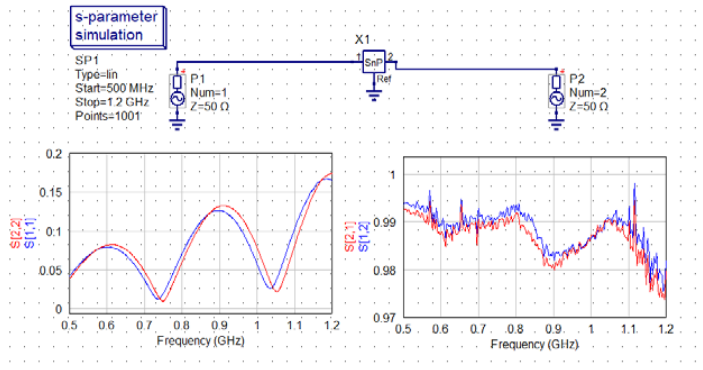
\includegraphics[width=0.9\linewidth]{Imagens/touchstone_validation.png}
    \caption{Validation of the Touchstone file in QucsStudio.}
    \label{fig:touchstone}
\end{figure}

When the PCB Touchstone model was combined with the antenna, a deterioration of the VSWR was observed, confirming the parasitic loading effect, as shown in Figure \ref{cap3:sec6:fig1585}. An updated matching network was therefore designed to restore the input impedance close to $50\,\Omega$. Figure~\ref{fig:matching_results} compares the results obtained in QucsStudio and SimNEC after optimisation.

\begin{figure}[H]
\centering
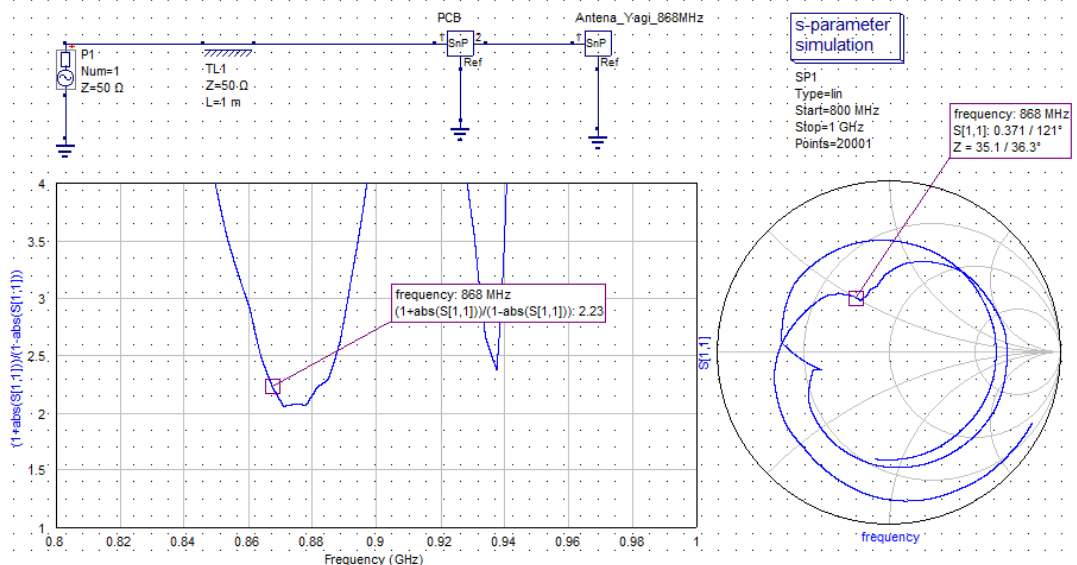
\includegraphics[width=0.9\linewidth]{Imagens/antena antes.png}
\caption{before impedance matching network.}
\label{cap3:sec6:fig1585}
\end{figure}

\begin{figure}[H]
    \centering
    \begin{subfigure}{0.8\textwidth}
        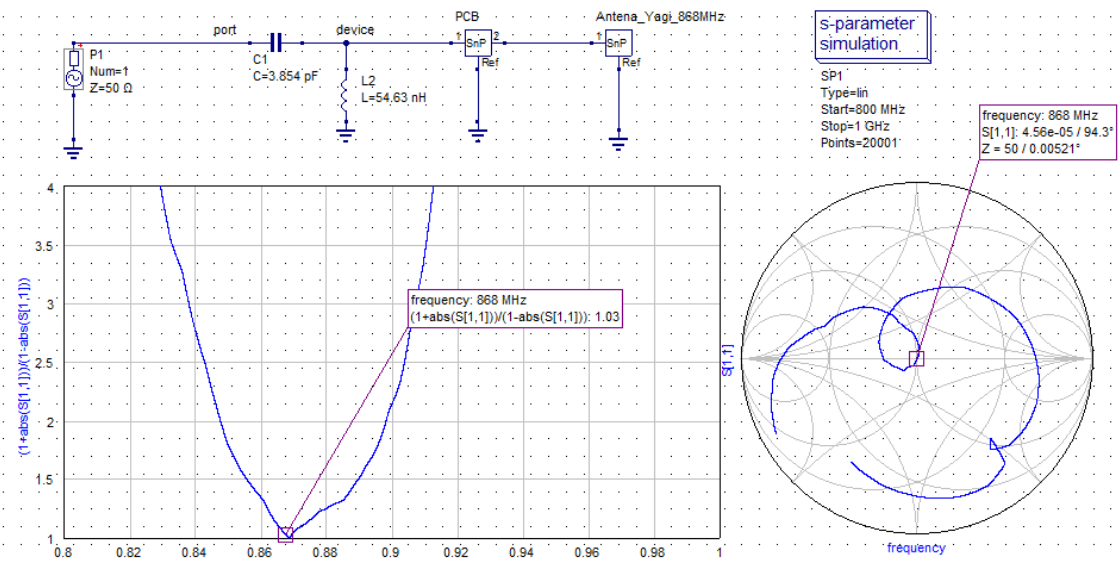
\includegraphics[width=\linewidth]{Imagens/antena depois.png}
        \caption{Impedance matching in QucsStudio.}
    \end{subfigure}\hfill
    \begin{subfigure}{0.8\textwidth}
        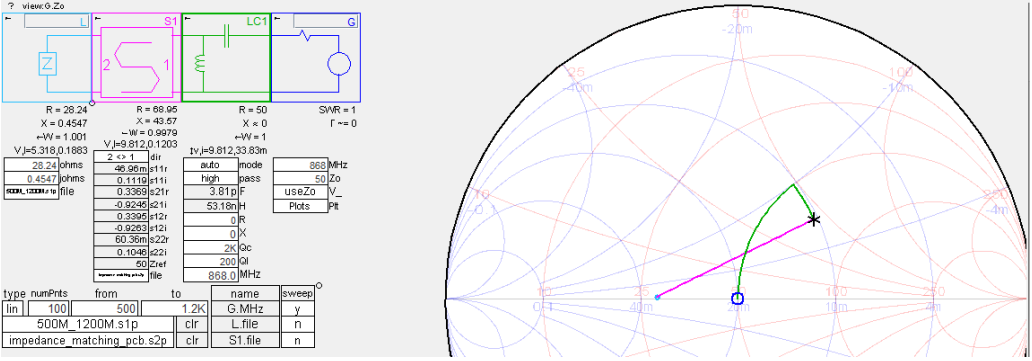
\includegraphics[width=\linewidth]{Imagens/Simnec_Matching.png}
        \caption{Matching network validation in SimNEC.}
    \end{subfigure}
    \caption{Results of the optimised matching network.}
    \label{fig:matching_results}
\end{figure}

The final values of network component are listed in Table~\ref{tab:lc_values}. These elements were used in the manufactured PCB.

\begin{table}[H]
\centering
\caption{Final LC matching network component values.}
\label{tab:lc_values}
\begin{tabular}{|l|c|c|}
\hline
Element & Estimated & Used \\ \hline
$L$     & 54.6~nH   & 56~nH \\ \hline
$C$     & 3.8~pF    & 3.9~pF \\ \hline
\end{tabular}
\end{table}


Finally, Figure~\ref{cap3:sec7:fig3} shows the complete PCB design workflow: (a) layout model in QucsStudio, (b) schematic design in EasyEDA\footnote{EasyEDA is a free, online PCB design software.}, and (c) the manufactured board.

\begin{figure}[H]
    \centering
    \begin{subfigure}{\textwidth}
        \centering
        \fbox{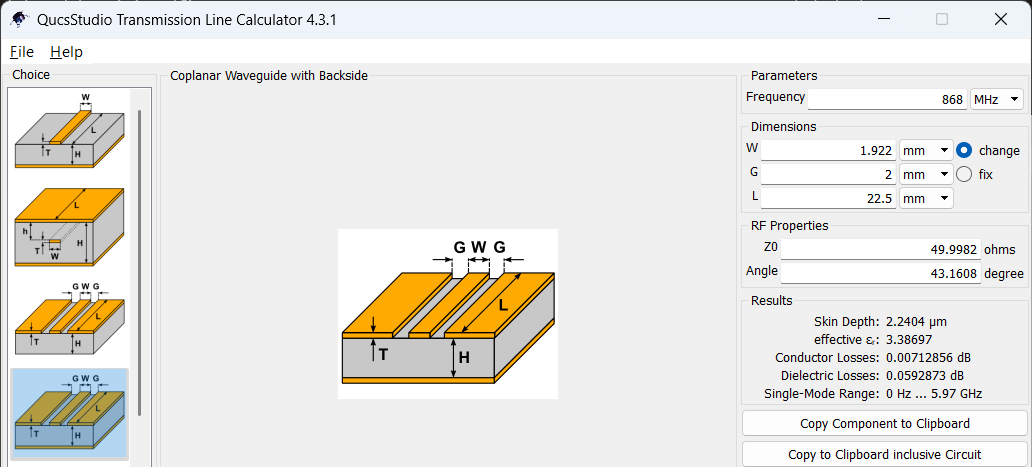
\includegraphics[width=0.6\linewidth]{Imagens/calculo da placa.png}}
        \caption{QucsStudio PCB layout model}
        \label{cap3:sec7:fig3:a}
    \end{subfigure}
    \vskip 2mm
    \begin{subfigure}{\textwidth}
        \centering
        \fbox{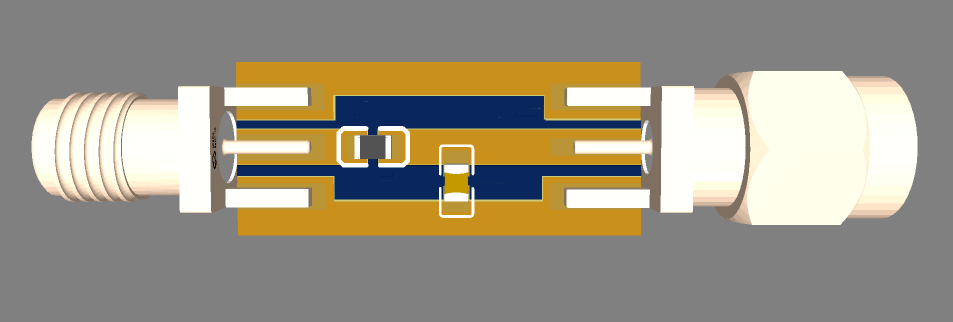
\includegraphics[width=0.6\linewidth]{Imagens/PCB3.png}}
        \caption{PCB design in EasyEDA}
        \label{cap3:sec7:fig3:b}
    \end{subfigure}
    \vskip 2mm
    \begin{subfigure}{\textwidth}
        \centering
        \fbox{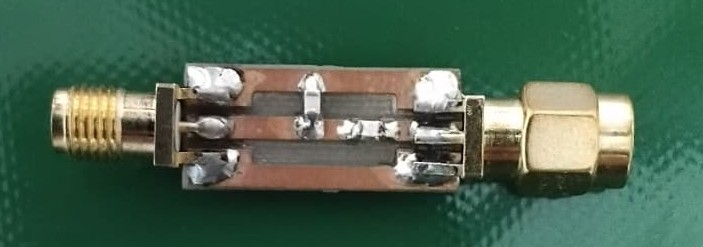
\includegraphics[width=0.6\linewidth]{Imagens/PCB_real.jpg}}
        \caption{Manufactured PCB photograph}
        \label{cap3:sec7:fig3:c}
    \end{subfigure}
    \caption{PCB layout model in QucsStudio , design in EasyEDA, and photograph of the manufactured.}
    \label{cap3:sec7:fig3}
\end{figure}


\section{Estimated Component Costs}
Table~\ref{tab:component_prices} summarises the average prices of the main components used in this project, both in Portugal and in the Asian market. Although these values are only indicative, they provide a realistic estimate of the typical costs involved. The total amount is modest, underscoring the low-cost nature of the design. When compared with the commercial equipment discussed in Chapter \ref{cap2:State_Of_The_Art}, the cost of this project represents only a small fraction.


\newpage

\begin{table}[H]
\centering
\caption{Estimated cost of components used in the project.}
\label{tab:component_prices}
\begin{tabular}{|l|c|c|}
\hline
\textbf{Component} & \textbf{Portugal} & \textbf{Asian Market} \\ \hline
Arduino UNO & \euro\;29.50 & \euro\;3.80 \\ \hline
Dual Bipolar Stepper Motor Shield for Arduino (DRV8825) & \euro\;34.50 & \euro\;6.80 \\ \hline
2 Hall-effect sensors & \euro\;5.38 & \euro\;0.44 \\ \hline
2 NEMA17 stepper motors & \euro\;24.00 & \euro\;16.54 \\ \hline
1.5 m GT2 timing belt (6 mm) & \euro\;3.60 & \euro\;2.58 \\ \hline
20-teeth pulley for NEMA17 stepper motor & \euro\;3.70 & \euro\;2.56 \\ \hline
Power supply 230V$\sim$12V - 2A & \euro\;4.97 & \euro\;4.68 \\ \hline
2 m fibreglass tube, 18 mm (12 mm inner) & \euro\;52.28 & \euro\;22.70 \\ \hline
1 Kg PLA filament (1.5 mm) & \euro\;15.49 & \euro\;7.00 \\ \hline
Electronic wires for connection & \euro\;15.52 & \euro\;6.32 \\ \hline
RF sensor detector & \euro\;20.70 & \euro\;8.58 \\ \hline
868 MHz band-pass filter & \euro\;14.95 & \euro\;5.57 \\ \hline
2 m copper rod (3 mm or 4 mm) & \euro\;7.60 & \euro\;4.25 \\ \hline
FR-4 copper-clad laminate (20X30 cm) & \euro\;6.96 & \euro\;5.24 \\ \hline
4 RF connector SMD (Male and Female) & \euro\;29.92 & \euro\;4.92 \\ \hline
Capacitor and Inductor SMD 0805  & \euro\;0.90 & \euro\;0.50 \\ \hline
Screws and Threads & \euro\;8.46 & \euro\;3.27 \\ \hline
2 nylon bearings & \euro\;3.86 & \euro\;1.35 \\ \hline
2 standard bearings & \euro3.94 & \euro\;3.15 \\ \hline
4 ball bearing with collar  & \euro\;15.25 & \euro\;3.85 \\ \hline
3 bases (wood or equivalent), Ø 30 cm & \euro\;4.80 & \euro\;8.10 \\ \hline
\textbf{TOTAL} & \textbf{\euro\;306.28} & \textbf{\euro\;122.20} \\ \hline
\end{tabular}
\end{table}

\indent The subsequent chapter presents the experimental results obtained and discusses their impact, considering the materials and methods described previously.